\documentclass[11pt,letterpaper]{article}


% pmml  arff  openannotation

%\usepackage[condensed,math]{anttor}
%\usepackage[T1]{fontenc}

%\usepackage[T1]{fontenc}
%\usepackage{tgtermes}

\usepackage[hang,flushmargin]{footmisc}

\usepackage{titlesec}

%\usepackage{sectsty}
%\sectionfont{\fontsize{13}{4}\selectfont}

\titleformat{\section}
  {\normalfont\fontsize{13}{15}\bfseries}{\thesection}{1em}{}

\titlespacing*{\section}
{0pt}{7ex plus 1ex minus .1ex}{2ex plus .2ex}

%\usepackage{mathptmx}

\usepackage{eso-pic}

%\setlength\parindent{0pt}

\AddToShipoutPictureBG{%

\ifnum\value{page}>1{
\AtTextUpperLeft{
\makebox[20.5cm][r]{
\raisebox{-1.95cm}{%
{\transparent{0.3}{
\includegraphics[width=0.29\textwidth]{e-logo.png}}	}} } }
}\fi
}

\AddToShipoutPicture{%
{
 {\color{blGreen!70!red}\transparent{0.9}{\put(0,0){\rule{3pt}{\paperheight}}}}%
 {\color{darkRed!70!purple}\transparent{1}\put(3,0){{\rule{4pt}{\paperheight}}}}
% {\color{logoPeach!80!cyan}\transparent{0.5}{\put(0,700){\rule{1cm}{.6cm}}}}%
% {\color{darkRed!60!cyan}\transparent{0.7}\put(0,706){{\rule{1cm}{.6cm}}}}
% \put(18,726){\thepage}
% \transparent{0.8}
}
}

\AddToShipoutPicture{%
\ifnum\value{page}>1
{\color{blGreen!70!red}\transparent{0.9}{\put(300,8){\rule{0.5\paperwidth}{.3cm}}}}%
{\color{inOne}\transparent{0.8}{\put(300,10){\rule{0.5\paperwidth}{.3cm}}}}%
{\color{inTwo}\transparent{0.3}\put(300,13){{\rule{0.5\paperwidth}{.3cm}}}}

{\color{blGreen!70!red}\transparent{0.9}{\put(5.6,5){\rule{0.5\paperwidth}{.4cm}}}}%
{\color{inOne}\transparent{1}{\put(5.6,10){\rule{0.5\paperwidth}{.4cm}}}}%
{\color{inTwo}\transparent{0.3}\put(5.6,15){{\rule{0.5\paperwidth}{.4cm}}}}

\put(301,16){%
\transparent{0.7}{

\includegraphics[width=0.2\textwidth]{logo.png}} }
\fi
}

\AddToShipoutPicture{%
\ifnum\value{page}=1
\put(257.5,729){%
	\transparent{0.7}{
		
\includegraphics[width=0.2\textwidth]{logo.png}}}
%\put(59,953){}
\fi
}	


%\pagestyle{empty} % no page number
%\parskip 7.2pt    % space between paragraphs
%\parindent 12pt   % indent for new paragraph
%\textwidth 4.5in  % width of text
%\columnsep 0.8in  % separation between columns

%\setlength{\footskip}{7pt}

\usepackage[paperheight=11in,paperwidth=8.5in]{geometry}
\geometry{left=.74in,top=.5in,right=.74in,bottom=1.2in} %margins

\usepackage{etoolbox}% http://ctan.org/pkg/etoolbox
\makeatletter
% \patchcmd{<cmd>}{<search>}{<replace>}{<success>}{<failure>}
\patchcmd{\@part}{\par}{\quad}{}{}
\patchcmd{\@part}{\huge}{\Large}{}{}
\makeatother

\renewcommand{\partname}{\hspace{-1em}Part}

\renewcommand*\thepart{\Roman{part}:}

\renewcommand{\thepage}{\raisebox{2pt}{\arabic{page}}}

\renewcommand{\footnoterule}{%
	\kern -3pt
	\hrule width .92\textwidth height .5pt
	\kern 10pt
}


\usepackage[hyphens]{url}
\newcommand{\biburl}[1]{ {\fontfamily{gar}\selectfont{\textcolor[rgb]{.2,.6,0}%
{\scriptsize {\url{#1}}}}}}

%\linespread{1.3}

\newcommand{\sectsp}{\vspace{12pt}}

\usepackage{graphicx}
\usepackage{color,framed}

\usepackage{textcomp}

\usepackage{float}

\usepackage{mdframed}


\usepackage{setspace}
\newcommand{\rpdfNotice}[1]{\begin{onehalfspacing}{

\Large #1

}\end{onehalfspacing}}

\usepackage{xcolor}

\usepackage[hyphenbreaks]{breakurl}
\usepackage[hyphens]{url}

\usepackage{hyperref}
\newcommand{\rpdfLink}[1]{\href{#1}{\small{#1}}}
\newcommand{\dblHref}[1]{\href{#1}{\small{\burl{#1}}}}
\newcommand{\browseHref}[2]{\href{#1}{\Large #2}}

\colorlet{blCyan}{cyan!50!blue}

\definecolor{darkRed}{rgb}{.2,.0,.1}


\definecolor{blGreen}{rgb}{.2,.7,.3}

\definecolor{darkBlGreen}{rgb}{.1,.3,.2}

\definecolor{oldBlColor}{rgb}{.2,.7,.3}

\definecolor{blColor}{rgb}{.1,.3,.2}

\definecolor{elColor}{rgb}{.2,.1,0}
\definecolor{flColor}{rgb}{0.7,0.3,0.3}

\definecolor{logoOrange}{RGB}{108, 18, 30}
\definecolor{logoGreen}{RGB}{85, 153, 89}
\definecolor{logoPurple}{RGB}{200, 208, 30}

\definecolor{logoBlue}{RGB}{4, 2, 25}
\definecolor{logoPeach}{RGB}{255, 159, 102}
\definecolor{logoCyan}{RGB}{66, 206, 244}
\definecolor{logoRed}{rgb}{.3,0,0}

\newcommand{\colorq}[1]{{\color{logoOrange!70!black}{\q{\small\textbf{#1}}}}}

\definecolor{inOne}{rgb}{0.122, 0.435, 0.698}% Rule colour
\definecolor{inTwo}{rgb}{0.122, 0.698, 0.435}% Rule colour

\definecolor{outOne}{rgb}{0.435, 0.698, 0.122}% Rule colour
\definecolor{outTwo}{rgb}{0.698, 0.435, 0.122}% Rule colour

\colorlet{linkcolor}{flColor!60!red}


\hypersetup{
	colorlinks=true,
	citecolor=blCyan!40!green,
	filecolor=magenta!30!logoBlue,
	urlcolor=blue,
    linkcolor=linkcolor!70!black,
%    allcolors=blCyan!40!green
}


\usepackage[many]{tcolorbox}% http://ctan.org/pkg/tcolorbox

\usepackage{transparent}

\newlength{\bsep}
\setlength{\bsep}{-1pt}
\let\xbibitem\bibitem
\renewcommand{\bibitem}[2]{\vspace{\bsep}\xbibitem{#1}{#2}}

\newenvironment{cframed}{\begin{mdframed}[linecolor=logoPeach,linewidth=0.4mm]}{\end{mdframed}}

\newenvironment{ccframed}{\begin{mdframed}[backgroundcolor=logoGreen!5,linecolor=logoCyan!50!black,linewidth=0.4mm]}{\end{mdframed}}


%\usepackage[T1]{fontenc}

%\usepackage{aurical}
% \Fontauri

\usepackage{gfsdidot}
\usepackage[T1]{fontenc}

%\makeatletter
%\f@family,  cmr, T1, n, m,
%\f@encoding,
%\f@shape,
%\f@series,
%\makeatother



%\usepackage{LibreBodoni}

%\usepackage{fontspec}
%\setmainfont{QTBengal}

\usepackage{relsize}

\newcommand{\bref}[1]{\hspace*{1pt}\textbf{\ref{#1}}}

\newcommand{\pseudoIndent}{

\vspace{10pt}\hspace*{12pt}}

\newcommand{\YPDFI}{{\fontfamily{fvs}\selectfont YPDF-Interactive}}

%
\newcommand{\deconum}[1]{{\protect\raisebox{-1pt}{{\LARGE #1}}}}

\newcommand{\visavis}{vis-\`a-vis}

\newcommand{\VersatileUX}{{\color{red!85!black}{\Fontauri Versatile}}%
{{\fontfamily{qhv}\selectfont\smaller UX}}}

\newcommand{\NDPCloud}{{\color{red!15!black}%
{\fontfamily{qhv}\selectfont {\smaller NDP C{\smaller LOUD}}}}}

\newcommand{\MThreeK}{{\color{blGreen!45!black}%
{\fontfamily{qhv}\fontsize{10}{8}\selectfont {M3K}}}}


\newcommand{\lfNDPCloud}{{\color{red!15!black}%
{\fontfamily{qhv}\selectfont N{\smaller DP C{\smaller LOUD}}}}}

\newcommand{\textds}[1]{{\fontfamily{lmdh}\selectfont{%
\raisebox{-1pt}{#1}}}}

%\newcommand{\dsC}{{\textds{ds}{\fontfamily{qhv}\selectfont \raisebox{-1pt}
%{\color{red!15!black}{C}}}}}

\definecolor{tcolor}{RGB}{24,52,61}



\newcommand{\ParaView}{\resizebox{!}{7pt}{\AcronymText{ParaView}}}
\newcommand{\Octave}{\resizebox{!}{7pt}{\AcronymText{Octave}}}
\newcommand{\ROOT}{\resizebox{!}{7pt}{\AcronymText{ROOT}}}
\newcommand{\CERN}{\resizebox{!}{7pt}{\AcronymText{CERN}}}
\newcommand{\MQFour}{\resizebox{!}{7pt}{\AcronymText{MQ4}}}
\newcommand{\VISSION}{\resizebox{!}{7pt}{\AcronymText{VISSION}}}



\newcommand{\CCpp}{\resizebox{!}{7pt}{\AcronymText{C}}/\Cpp{}}
\newcommand{\NoSQL}{\resizebox{!}{7pt}{\AcronymText{NoSQL}}}
\newcommand{\SQL}{\resizebox{!}{7pt}{\AcronymText{SQL}}}

\newcommand{\SPARQL}{\resizebox{!}{7pt}{\AcronymText{SPARQL}}}

\newcommand{\NCBI}{\resizebox{!}{7pt}{\AcronymText{NCBI}}}

\newcommand{\HTXN}{\resizebox{!}{7pt}{\AcronymText{HTXN}}}

\newcommand{\OWL}{\resizebox{!}{7pt}{\AcronymText{OWL}}}

\newcommand{\TDM}{\resizebox{!}{7pt}{\AcronymText{TDM}}}

\newcommand{\lHTXN}{\resizebox{!}{7.5pt}{\AcronymText{H}}%
\resizebox{!}{6.5pt}{\AcronymText{TXN}}}

\newcommand{\lsHTXN}{\resizebox{!}{9.5pt}{\AcronymText{\textcolor{tcolor}{HTXN}}}}

\newcommand{\LAF}{\resizebox{!}{7pt}{\AcronymText{LAF}}}

\newcommand{\UDpipe}{\resizebox{!}{7pt}{\AcronymText{UDpipe}}}

\newcommand{\C}{\resizebox{!}{7pt}{\AcronymText{C}}}


\usepackage{mdframed}

\newcommand{\cframedboxpanda}[1]{\begin{mdframed}[linecolor=yellow!70!blue,linewidth=0.4mm]#1\end{mdframed}}


\newcommand{\PVD}{\resizebox{!}{7pt}{\AcronymText{PVD}}}

\newcommand{\SDK}{\resizebox{!}{7pt}{\AcronymText{SDK}}}
\newcommand{\NLP}{\resizebox{!}{7pt}{\AcronymText{NLP}}}

\newcommand{\AXF}{\resizebox{!}{7pt}{\AcronymText{AXF}}}

\newcommand{\lAXF}{\resizebox{!}{7.5pt}{\AcronymText{A}}%
\resizebox{!}{6.5pt}{\AcronymText{XF}}}


\newcommand{\lsAXF}{\resizebox{!}{8.5pt}{\AcronymText{AXF}}}

\newcommand{\AXFD}{\resizebox{!}{7pt}{\AcronymText{AXFD}}}

\newcommand{\CBICA}{\resizebox{!}{7pt}{\AcronymText{CBICA}}}

\newcommand{\IORT}{\resizebox{!}{7pt}{\AcronymText{IORT}}}


\newcommand{\SeDI}{\resizebox{!}{7pt}{\AcronymText{SeDI}}}
\newcommand{\RSNA}{\resizebox{!}{7pt}{\AcronymText{RSNA}}}

\newcommand{\CER}{\resizebox{!}{7pt}{\AcronymText{CER}}}
\newcommand{\PACS}{\resizebox{!}{7pt}{\AcronymText{PACS}}}

\newcommand{\DICOM}{\resizebox{!}{7pt}{\AcronymText{DICOM}}}

\newcommand{\CT}{\resizebox{!}{7pt}{\AcronymText{CT}}}

\newcommand{\LOINC}{\resizebox{!}{7pt}{\AcronymText{LOINC}}}


\newcommand{\TAGML}{\resizebox{!}{7pt}{\AcronymText{TAGML}}}

\newcommand{\CPAP}{\resizebox{!}{7pt}{\AcronymText{CPAP}}}

\newcommand{\RadLex}{\resizebox{!}{7pt}{\AcronymText{RadLex}}}


\newcommand{\OMOP}{\resizebox{!}{7pt}{\AcronymText{OMOP}}}
\newcommand{\PCORnet}{\resizebox{!}{7pt}{\AcronymText{PCORnet}}}
\newcommand{\FHIR}{\resizebox{!}{7pt}{\AcronymText{FHIR}}}

\newcommand{\CaPTk}{\resizebox{!}{7pt}{\AcronymText{CaPTk}}}

\newcommand{\VIOLIN}{\resizebox{!}{7pt}{\AcronymText{VIOLIN}}}



\newcommand{\lAXFD}{\resizebox{!}{7.5pt}{\AcronymText{A}}%
\resizebox{!}{6.5pt}{\AcronymText{XFD}}}


\newcommand{\IJST}{\resizebox{!}{7pt}{\AcronymText{IJST}}}

\newcommand{\Jupyter}{\resizebox{!}{7pt}{\AcronymText{Jupyter}}}
\newcommand{\Python}{\resizebox{!}{7pt}{\AcronymText{Python}}}
\newcommand{\IDN}{\resizebox{!}{7pt}{\AcronymText{IDN}}}
\newcommand{\JPG}{\resizebox{!}{7pt}{\AcronymText{JPG}}}
\newcommand{\PNG}{\resizebox{!}{7pt}{\AcronymText{PNG}}}
\newcommand{\TIFF}{\resizebox{!}{7pt}{\AcronymText{TIFF}}}
\newcommand{\REPL}{\resizebox{!}{7pt}{\AcronymText{REPL}}}


\newcommand{\BioC}{\resizebox{!}{7pt}{\AcronymText{BioC}}}

\newcommand{\CoNLL}{\resizebox{!}{7pt}{\AcronymText{CoNLL}}}
\newcommand{\CoNLLU}{\resizebox{!}{7pt}{\AcronymText{CoNLL-U}}}

\newcommand{\sapp}{\resizebox{!}{7pt}{\AcronymText{Sapien+}}}
\newcommand{\lsapp}{\resizebox{!}{8.5pt}{\AcronymText{Sapien+}}}
\newcommand{\lssapp}{\resizebox{!}{9.5pt}{\AcronymText{Sapien+}}}

\newcommand{\ePub}{\resizebox{!}{7pt}{\AcronymText{ePub}}}

%\lsLPF


\newcommand{\GIT}{\resizebox{!}{7pt}{\AcronymText{GIT}}}

%\definecolor{atColor}{RGB}{11, 71, 17}


\DeclareMathVersion{fordg}
\SetSymbolFont{letters}{fordg}{OML}{cmr}{b}{n}

\definecolor{atcColor}{RGB}{96, 17, 12}
\newcommand{\ATextCClr}[1]{\textcolor{atcColor}{\textbf{#1}}}

\newcommand{\AIMConc}{\resizebox{!}{7.5pt}{\ATextCClr{AIM-Concepts}}}
\newcommand{\lAIMConc}{\resizebox{!}{8pt}{\ATextCClr{AIM-Concepts}}}

\newcommand{\HGXF}{{\resizebox{!}{7.5pt}{\ATextCClr{HGXF}}}}
\newcommand{\lHGXF}{{\resizebox{!}{8pt}{\ATextCClr{HGXF}}}}
\newcommand{\sHGXF}{{\resizebox{!}{6pt}{\ATextCClr{HGXF}}}}

\newcommand{\MdsX}{\resizebox{!}{7.5pt}{\ATextCClr{MdsX}}}
\newcommand{\lsMdsX}{\resizebox{!}{9pt}{\ATextCClr{MdsX}}}


\newcommand{\HMCL}{{\resizebox{!}{7.5pt}{\ATextCClr{HMCL}}}}
\newcommand{\DSPIN}{{\resizebox{!}{7.5pt}{\ATextCClr{D-SPIN}}}}


\newcommand{\CRtwo}{{\resizebox{!}{7.5pt}{\ATextCClr{CR2}}}}
\newcommand{\lCRtwo}{{\resizebox{!}{8pt}{\ATextCClr{CR2}}}}
\newcommand{\sCRtwo}{{\resizebox{!}{6pt}{\ATextCClr{CR2}}}}


\newcommand{\THQL}{\resizebox{!}{7.5pt}{\ATextCClr{THQL}}}
\newcommand{\lTHQL}{\resizebox{!}{8pt}{\ATextCClr{THQL}}}

\newcommand{\HDICOM}{\resizebox{!}{7.5pt}{\ATextCClr{{\large h}-DICOM}}}

\newcommand{\hVaImm}{\resizebox{!}{7.5pt}{\ATextCClr{{\large h}-VaImm}}}


\newcommand{\PhaonVI}{\resizebox{!}{7.5pt}{\ATextCClr{Phaon-VI}}}



\definecolor{atColor}{RGB}{50, 22, 40}
\newcommand{\ATextClr}[1]{\textcolor{atColor}{\textbf{#1}}}

\newcommand{\DgDb}{{\mathversion{fordg}%
\makebox{\raisebox{-3pt}{\resizebox{!}{11pt}{\ATextClr{%
\rotatebox{17}{$\varsigma$}}}}\hspace{-4pt}%
\resizebox{!}{6.5pt}{\ATextClr{D\hspace{-2pt}B}}}}}


\newcommand{\lDgDb}{{\mathversion{fordg}%
\resizebox{!}{12pt}{\ATextClr{%
\rotatebox{17}{$\varsigma$}}}}\hspace{-4pt}%
\resizebox{!}{6.5pt}{\ATextClr{D\hspace{-2pt}B}}}}}

\newcommand{\URL}{\resizebox{!}{7pt}{\AcronymText{URL}}}
\newcommand{\CSML}{\resizebox{!}{7pt}{\AcronymText{CSML}}}
\newcommand{\LPF}{\resizebox{!}{7pt}{\AcronymText{LPF}}}
\newcommand{\lLPF}{\resizebox{!}{8.5pt}{\AcronymText{LPF}}}
\newcommand{\lsLPF}{\resizebox{!}{9.5pt}{\AcronymText{LPF}}}

\newcommand{\AI}{\resizebox{!}{7.5pt}{\AcronymText{AI}}}
\newcommand{\lAI}{\resizebox{!}{8pt}{\AcronymText{AI}}}

\makeatletter

\newcommand*\getX[1]{\expandafter\getX@i#1\@nil}

\newcommand*\getY[1]{\expandafter\getY@i#1\@nil}
\def\getX@i#1,#2\@nil{#1}
\def\getY@i#1,#2\@nil{#2}
\makeatother
	
\newcommand{\rectann}[9]{%
\path [draw=#1,draw opacity=#2,line width=#3, fill=#4, fill opacity = #5, even odd rule] %
(#6) rectangle(\getX{#6}+#7,\getY{#6}+#8)
({\getX{#6}+((#7-(#7*#9))/2)},{\getY{#6}+((#8-(#8*#9))/2)}) rectangle %
({\getX{#6}+((#7-(#7*#9))/2)+#7*#9},{\getY{#6}+((#8-(#8*#9))/2)+#8*#9});}


\definecolor{pfcolor}{RGB}{94, 54, 73}

\newcommand{\EPF}{\resizebox{!}{7pt}{\AcronymText{ETS{\color{pfcolor}pf}}}}
\newcommand{\lEPF}{\resizebox{!}{8.5pt}{\AcronymText{ETS{\color{pfcolor}pf}}}}
\newcommand{\lsEPF}{\resizebox{!}{9.5pt}{\AcronymText{ETS{\color{pfcolor}pf}}}}


\newcommand{\XPDF}{\resizebox{!}{7pt}{\AcronymText{XPDF}}}

\newcommand{\GRE}{\resizebox{!}{7pt}{\AcronymText{GRE}}}
\newcommand{\CAS}{\resizebox{!}{7pt}{\AcronymText{CAS}}}

\newcommand{\lMOSAIC}{%
\resizebox{!}{8pt}{\AcronymText{M}}%
\resizebox{!}{6pt}{\AcronymText{OSAIC}}}

\newcommand{\XML}{\resizebox{!}{7pt}{\AcronymText{XML}}}
\newcommand{\RDF}{\resizebox{!}{7pt}{\AcronymText{RDF}}}
\newcommand{\DOM}{\resizebox{!}{7pt}{\AcronymText{DOM}}}

\newcommand{\Covid}{\resizebox{!}{7pt}{\AcronymText{Covid-19}}}

\newcommand{\CLang}{\resizebox{!}{7pt}{\AcronymText{C}}}

\newcommand{\HNaN}{\resizebox{!}{7pt}{\AcronymText{HN%
\textsc{a}N}}}

\newcommand{\JSON}{\resizebox{!}{7pt}{\AcronymText{JSON}}}
\newcommand{\UV}{\resizebox{!}{7pt}{\AcronymText{UV}}}


\newcommand{\MeshLab}{\resizebox{!}{7pt}{\AcronymText{MeshLab}}}
\newcommand{\IQmol}{\resizebox{!}{7pt}{\AcronymText{IQmol}}}

\newcommand{\SGML}{\resizebox{!}{7pt}{\AcronymText{SGML}}}

\newcommand{\WhiteDB}{\makebox{WhiteDB}}

\newcommand{\ASCII}{\resizebox{!}{7pt}{\AcronymText{ASCII}}}

\newcommand{\DSPIN}{\resizebox{!}{7pt}{\AcronymText{D-SPIN}}}


\newcommand{\GUI}{\resizebox{!}{7pt}{\AcronymText{GUI}}}

\newcommand{\URI}{\resizebox{!}{7pt}{\AcronymText{URI}}}
\newcommand{\DTD}{\resizebox{!}{7pt}{\AcronymText{DTD}}}

\newcommand{\API}{\resizebox{!}{7pt}{\AcronymText{API}}}

\newcommand{\JATS}{\resizebox{!}{7pt}{\AcronymText{JATS}}}


\newcommand{\SDI}{\resizebox{!}{7pt}{\AcronymText{SDI}}}
\newcommand{\SDIV}{\resizebox{!}{7pt}{\AcronymText{SDIV}}}

\definecolor{atColor}{RGB}{50, 22, 40}
\newcommand{\ATextClr}[1]{\textcolor{atColor}{\textbf{#1}}}

\newcommand{\DgDb}{\makebox{\raisebox{-3pt}{\resizebox{!}{11pt}{\ATextClr{%
\rotatebox{17}{$\varsigma$}}}}\hspace{-4pt}%
\resizebox{!}{6.5pt}{\ATextClr{D\hspace{-2pt}B}}}}

\newcommand{\lDgDb}{\makebox{\raisebox{-3pt}{%
\resizebox{!}{12pt}{\ATextClr{%
\rotatebox{17}{$\varsigma$}}}}\hspace{-4pt}%
\resizebox{!}{6.5pt}{\ATextClr{D\hspace{-2pt}B}}}}


\newcommand{\IDE}{\resizebox{!}{7pt}{\AcronymText{IDE}}}


\newcommand{\ViSion}{\resizebox{!}{7pt}{\AcronymText{ViSion}}}

\newcommand{\CWL}{\resizebox{!}{7pt}{\AcronymText{CWL}}}

\newcommand{\ThreeD}{\resizebox{!}{7pt}{\AcronymText{3D}}}
\newcommand{\TwoD}{\resizebox{!}{7pt}{\AcronymText{2D}}}

\newcommand{\medInria}{\resizebox{!}{7pt}{\AcronymText{medInria}}}
\newcommand{\ThreeDimViewer}{\resizebox{!}{7pt}{\AcronymText{3DimViewer}}}

\newcommand{\FAIR}{\resizebox{!}{7pt}{\AcronymText{FAIR}}}

\newcommand{\QNetworkManager}{\resizebox{!}{7pt}{\AcronymText{QNetworkManager}}}
\newcommand{\QTextDocument}{\resizebox{!}{7pt}{\AcronymText{QTextDocument}}}
\newcommand{\QWebEngineView}{\resizebox{!}{7pt}{\AcronymText{QWebEngineView}}}
\newcommand{\HTTP}{\resizebox{!}{7pt}{\AcronymText{HTTP}}}


\newcommand{\lAcronymTextNC}[2]{{\fontfamily{fvs}\selectfont {\Large{#1}}{\large{#2}}}}

\newcommand{\AcronymTextNC}[1]{{\fontfamily{fvs}\selectfont {\large #1}}}


\colorlet{orr}{orange!60!red}

\newcommand{\textscc}[1]{{\color{orr!35!black}{{%
						\fontfamily{Cabin-TLF}\fontseries{b}\selectfont{\textsc{\scriptsize{#1}}}}}}}


\newcommand{\textsccserif}[1]{{\color{orr!35!black}{{%
				\scriptsize{\textbf{#1}}}}}}


\newcommand{\iXPDF}{\resizebox{!}{7pt}{\textsccserif{%
\textit{XPDF}}}}

\newcommand{\iEPF}{\resizebox{!}{7pt}{\textsccserif{%
\textit{ETSpf}}}}

\newcommand{\iSDI}{\resizebox{!}{7pt}{\textsccserif{%
\textit{SDI}}}}

\newcommand{\iHTXN}{\resizebox{!}{7pt}{\textsccserif{%
\textit{HTXN}}}}


\newcommand{\AcronymText}[1]{{\textscc{#1}}}

\newcommand{\AcronymTextser}[1]{{\textsccserif{#1}}}


\newcommand{\mAcronymText}[1]{{\textscc{\normalsize{#1}}}}

\newcommand{\FASTA}{{\resizebox{!}{7pt}{\AcronymText{FASTA}}}}
\newcommand{\SRA}{{\resizebox{!}{7pt}{\AcronymText{SRA}}}}
\newcommand{\DNA}{{\resizebox{!}{7pt}{\AcronymText{DNA}}}}
\newcommand{\MAP}{{\resizebox{!}{7pt}{\AcronymText{MAP}}}}
\newcommand{\EPS}{{\resizebox{!}{7pt}{\AcronymText{EPS}}}}
\newcommand{\CSV}{{\resizebox{!}{7pt}{\AcronymText{CSV}}}}
\newcommand{\PDB}{{\resizebox{!}{7pt}{\AcronymText{PDB}}}}


\newcommand{\OBO}{{\resizebox{!}{7pt}{\AcronymText{OBO}}}}

\newcommand{\XOCS}{{\resizebox{!}{7pt}{\AcronymText{XOCS}}}}

\newcommand{\ChemXML}{{\resizebox{!}{7pt}{\AcronymText{ChemXML}}}}

\newcommand{\TeXMECS}{\resizebox{!}{7pt}{\AcronymText{TeXMECS}}}

% pmml  arff  openannotation

\newcommand{\PMML}{\resizebox{!}{7pt}{\AcronymText{PMML}}}
\newcommand{\ARFF}{\resizebox{!}{7pt}{\AcronymText{ARFF}}}
\newcommand{\IeXML}{\resizebox{!}{7pt}{\AcronymText{IeXML}}}


\newcommand{\WebGL}{\resizebox{!}{7pt}{\AcronymText{WebGL}}}


\newcommand{\Cpp}{\resizebox{!}{7pt}{\AcronymText{C++}}}

%\newcommand{\\WhiteDB{}}{\resizebox{!}{7pt}{\AcronymText{\WhiteDB{}}}}

\colorlet{drp}{darkRed!70!purple}

%\newcommand{\MOSAIC}{{\color{drp}{\AcronymTextNC{\scriptsize{MOSAIC}}}}}

\newcommand{\MOSAIC}{\resizebox{!}{7pt}{\AcronymText{MOSAIC}}}


\newcommand{\mMOSAIC}{{\color{drp}{\AcronymTextNC{\normalsize{MOSAIC}}}}}

\newcommand{\MOSAICVM}{\mMOSAIC-\mAcronymText{VM}}

\newcommand{\sMOSAICVM}{\resizebox{!}{7pt}{\MOSAICVM}}
\newcommand{\sMOSAIC}{\resizebox{!}{7pt}{\MOSAIC}}

\newcommand{\LDOM}{\resizebox{!}{7pt}{\AcronymText{LDOM}}}
\newcommand{\Cnineteen}{\resizebox{!}{7pt}{\AcronymText{CORD-19}}}

\newcommand{\lCnineteen}{\resizebox{!}{7.5pt}{\AcronymText{CORD-19}}}


\newcommand{\MOL}{\resizebox{!}{7pt}{\AcronymText{MOL}}}

\newcommand{\ACL}{\resizebox{!}{7pt}{\AcronymText{ACL}}}

\newcommand{\LXCR}{\resizebox{!}{7pt}{\AcronymText{LXCR}}}
\newcommand{\lLXCR}{\resizebox{!}{8.5pt}{\AcronymText{LXCR}}}
\newcommand{\lsLXCR}{\resizebox{!}{9.5pt}{\AcronymText{LXCR}}}

%\newcommand{\lMOSAIC}{{\color{drp}{\lAcronymTextNC{M}{OSAIC}}}}
\newcommand{\lfMOSAIC}{\resizebox{!}{9pt}{{\color{drp}{\lAcronymTextNC{M}{OSAIC}}}}}

\newcommand{\Mosaic}{\resizebox{!}{7pt}{\MOSAIC}}
\newcommand{\MosaicPortal}{{\color{drp}{\AcronymTextNC{MOSAIC Portal}}}}

\newcommand{\RnD}{\resizebox{!}{7pt}{\AcronymText{R\&D}}}

\newcommand{\lQt}{\resizebox{!}{8.5pt}{\AcronymText{Qt}}}
\newcommand{\QtCpp}{\resizebox{!}{8.5pt}{\AcronymText{Qt/C++}}}
\newcommand{\Qt}{\resizebox{!}{7pt}{\AcronymText{Qt}}}

\newcommand{\QtSQL}{\resizebox{!}{7pt}{\AcronymText{QtSQL}}}

\newcommand{\HTML}{\resizebox{!}{7pt}{\AcronymText{HTML}}}
\newcommand{\PDF}{\resizebox{!}{7pt}{\AcronymText{PDF}}}

\newcommand{\R}{\resizebox{!}{7pt}{\AcronymText{R}}}
\newcommand{\SciXML}{\resizebox{!}{7pt}{\AcronymText{SciXML}}}



\newcommand{\lGRE}{\resizebox{!}{7.5pt}{\AcronymText{GRE}}}

\newcommand{\p}[1]{

\vspace{1em}#1}

\newcommand{\q}[1]{{\fontfamily{qcr}\selectfont ``}#1{\fontfamily{qcr}\selectfont ''}} 

%\newcommand{\deconum}[1]{{\textcircled{#1}}}

\renewcommand{\thesection}{\protect\hspace{-1.5em}}
%\renewcommand{\thesection}{\protect\mbox{\deconum{\Roman{section}}}}
\renewcommand{\thesubsection}{\arabic{section}.\arabic{subsection}}

\newcommand{\llMOSAIC}{\mbox{{\LARGE MOSAIC}}}
%\newcommand{\lfMOSAIC}{\mbox{M\small{OSAIC}}}

\newcommand{\llMosaic}{\llMOSAIC}
\newcommand{\lMosaic}{\lMOSAIC}
\newcommand{\lfMosaic}{\lfMOSAIC}

%\newcommand{\dsC}{}

\newcommand{\textds}[1]{{\fontfamily{lmdh}\selectfont{%
\raisebox{-1pt}{#1}}}}

\newcommand{\ltextds}[1]{{\fontfamily{lmdh}\fontsize{12}{11}\selectfont{%
\raisebox{-1pt}{#1}}}}

\newcommand{\dsC}{{\textds{ds}{\fontfamily{qhv}\selectfont \raisebox{-1pt}{C}}}}
\newcommand{\ldsC}{{\textds{ds}{\fontfamily{qhv}\selectfont \raisebox{-1pt}{C}}}}

\newcommand{\llWC}{\mbox{{\LARGE WhiteCharmDB}}}

\newcommand{\llwh}{\mbox{{\LARGE White}}}
\newcommand{\llch}{\mbox{{\LARGE CharmDB}}}

\usepackage{enumitem}
%\usepackage{listings}

\colorlet{dsl}{purple!20!brown}
\colorlet{dslr}{dsl!50!blue}

\setlist[description]{%
  topsep=11pt,
  labelsep=22pt, leftmargin=10pt,
  itemsep=13pt,               % space between items
  %font={\bfseries\sffamily}, % set the label font
  font=\normalfont\bfseries\color{dslr!50!black}, % if colour is needed
}

\setlist[enumerate]{%
  topsep=3pt,               % space before start / after end of list
  itemsep=-2pt,               % space between items
  font={\bfseries\sffamily}, % set the label font
%  font={\bfseries\sffamily\color{red}}, % if colour is needed
}

%\usepackage{tcolorbox}

\newcommand{\slead}[1]{%
\noindent{\raisebox{2pt}{\relscale{1.15}{{{%
\fcolorbox{logoCyan!50!black}{logoGreen!5}{#1}
}}}}}\hspace{.5em}}


\let\OldLaTeX\LaTeX

\renewcommand{\LaTeX}{\resizebox{!}{7pt}{\color{orr!35!black}{\OldLaTeX}}}

\let\OldTeX\TeX

\renewcommand{\TeX}{\resizebox{!}{7pt}{\color{orr!35!black}{\OldTeX}}}


\newcommand{\LargeLaTeX}{\resizebox{!}{8.5pt}{\color{orr!35!black}{\OldLaTeX}}}

%\setlength\parindent{0pt}
\setlength\parindent{24pt}
%
\usepackage{titlesec}
\usepackage[hyphens]{url}

\newsavebox{\tempbox}
\sbox{\tempbox}{\raisebox{-4.5pt}%
{\parbox{3cm}{\textit{\textbf{{\large ``Channel \hspace{1em} Abstractions"}}}}}}

%\newsavebox{\sstwolinebox}
%\sbox{\sstwolinebox}{\raisebox{-5pt}%
%{\parbox{7.4cm}{\textit{\textbf{{\large %
%Range-Bounded Types, Value Constructors, and Addressability}}}}}}
%\newcommand{\sstwoline}{\usebox{\sstwolinebox}}

%\definecolor{midRed}{rgb}{.5,.0,.25}
%\definecolor{logoRed}{rgb}{.3,0,0}



\newenvironment{displayquotexxx}{%
	%\begin{fcolorbox}{yellow!20!gray}{red!5}
	\begin{flushright}
	\begin{tcolorbox}[
		colback=gray!4,
		colframe=red!20!gray,
		width=.98\linewidth,
		boxrule=1pt,leftrule=3pt,
		rightrule=1pt,toprule=.5pt,arc=0pt,auto outer arc
		]
\begin{minipage}{21.5em}}{%
\end{minipage}\end{tcolorbox}
	\end{flushright}
}

\usepackage{changepage}

\newenvironment{dquote}{%
	%\begin{fcolorbox}{yellow!20!gray}{red!5}
	\begin{flushright}
	\vspace{1em}\begin{tcolorbox}[
		breakable, parbox=false, colback=gray!4,
		colframe=mRed!20!gray,
		width=.995\linewidth,
		boxrule=1pt,leftrule=3pt,
		rightrule=1pt,toprule=.5pt,arc=0pt,auto outer arc
		]
\begin{adjustwidth}{1pt}{-3pt}
}{%
\end{adjustwidth}
\end{tcolorbox}\vspace{1em}
	\end{flushright}
}



\newcounter{subs}[section]

\newcommand{\subss}[2]{	
\phantomsection \label{#1}
\addcontentsline{toc}{subsection}{#1}
\stepcounter{subs}
\refstepcounter{subsection}
\vspace*{3.25em}

\noindent{ {\Large\textbf\thesection.}{\large\textbf\thesubs}} {
 {{\Large\textbf #2}}
}
\vspace*{.35em} 
}

\newcommand{\subsstlx}[2]{}

\newcommand{\subsstl}[2]{	
\phantomsection \label{#1}
\addcontentsline{toc}{subsection}{#1}
\stepcounter{subs}
\refstepcounter{subsection}
\vspace*{3.25em}

\noindent{ \raisebox{-1pt}{\Large\textbf\thesection.}{\large\textbf\thesubs}} {
\raisebox{-1pt}{{\Large\textbf #2}}
}
\vspace*{.35em} 
}

\newcommand{\subsstly}[2]{	
\phantomsection \label{#1}
\addcontentsline{toc}{subsection}{#1}
\stepcounter{subs}
\refstepcounter{subsection}
\vspace*{3.25em}

\noindent{ \raisebox{-1pt}{\Large\textbf\thesection.}{\large\textbf\thesubs}} {
\raisebox{-1pt}{{\Large\textbf #2}}
}
\vspace*{.35em} 
}


\let\Osubsection\subsection

\renewcommand{\subsection}[1]{\subss{#1}{#1}}

\newcommand{\subsectionalt}[2]{\subss{#1}{#2}}


\newsavebox{\twolinebox}

\newcommand{\stwoline}[1]{%
\sbox{\twolinebox}{\raisebox{-3pt}%
{\parbox{7.4cm}{\linespread{1.25}\selectfont\raggedleft{\textbf{{\large #1}}}}}}}

\newcommand{\twoline}{\usebox{\twolinebox}}

\newcommand{\subsectiontwoline}[1]{\stwoline{#1}\subsstl{#1}{\twoline}

\vspace{1em}}

\newcommand{\spsubsectiontwolinerepl}[2]{\stwoline{#1}\subsstl{#2}{\twoline}}
\newcommand{\subsectiontwolinerepl}[2]{\stwoline{#1}\subsstl{#2}{\twoline}

\vspace{1em}}

\newcommand{\subsectiontwolinealt}[2]{\stwoline{#1}\subsstl{#2}{\twoline}

\vspace{1em}}


\titlespacing{\subsection}{0pt}{20pt}{20pt}
\titlespacing{\section}{0pt}{35pt}{15pt}
\titlespacing{\subsubsection}{0pt}{20pt}{5pt}


\newcommand{\spsubsection}[1]{%
\subss{#1}{#1}
\vspace{1em}
}
\newcommand{\spsubsectiontwoline}[1]{%
\subsectiontwoline{#1}
\vspace{1em}
}



\usepackage{csquotes}

\usepackage{booktabs}

\usepackage{amssymb}

\usepackage{titlesec}

\usepackage{transparent}

\usepackage{setspace}

\usepackage{graphicx}

\newcommand{\sectionGraphics}{

\vspace{2em}\centerline{\includegraphics[scale=0.125]{logo-deco.png}}\vspace{-1em}}

\usepackage[flushmargin]{footmisc}

\setlength{\parindent}{30pt}

\usepackage[letterpaper, left=.47in,right=.47in,top=.825in,bottom=.825in]{geometry}

\let\xbibitem\bibitem
\renewcommand{\bibitem}[2]{\vspace{6.5pt}\xbibitem{#1}{#2}}

\newenvironment{frquote}{%
%\begin{fcolorbox}{yellow!20!gray}{red!5}
%\begin{flushright}

\begin{tcolorbox}[
	colback=white,
	colframe=white,
	width=.97\linewidth,
	arc=0mm, auto outer arc
	]
\begin{scriptsize}
\begin{minipage}{61em}
\begin{flushright}
\begin{minipage}{63em}}{%
\end{minipage}
\end{flushright}
\end{minipage}
\end{scriptsize}
\end{tcolorbox}
%\end{flushright}
}

%\colorlet{codegr}{black!80!blue}

\setlength{\columnsep}{8mm}

\usepackage{etoolbox}

\AtBeginEnvironment{thebibliography}{\linespread{1}\selectfont}

\usepackage{mathptmx}

\titleformat*{\subsection}{\small\bfseries}

\usepackage{wasysym}
\usepackage{textcomp}
\usepackage{amssymb}

\usepackage{microtype}

\DeclareMathAlphabet{\mathcal}{OMS}{cmsy}{m}{n}

\let\OldI\i

\newcommand{\secvspace}{\vspace{-0.3em}}
\newcommand{\asecvspace}{\vspace{-0.05em}}

\newcommand{\mdash}{---}
\newcommand{\q}[1]{``#1"}
\newcommand{\sq}[1]{`#1'}
\renewcommand{\i}[1]{\textit{#1}}

\newcommand{\nl}{

}

\newcommand{\T}[1]{\raisebox{-2pt}{\ensuremath{\mathcal{T}}}\textit{\tiny #1}}

\newcommand{\biburl}[1]{ {\fontfamily{gar}\selectfont{\textcolor[rgb]{.2,.6,0}%
{\scriptsize {\url{#1}}}}}}

%\newcommand{\biburl}[1]{ {\fontfamily{gar}\selectfont{\textcolor[rgb]%%{.2,.6,0}%
%{\scriptsize \textls*[-70]{\burl{#1}}}}}}

\newcommand{\TSupT}{\ensuremath{{\T2}\makebox[4pt][r]{\raisebox{5pt}{{\scalebox{.6}{\T1}}}}}}

\let\OldFootnoteSize\footnotesize
\renewcommand{\footnotesize}{\scriptsize}

\newcommand{\emigres}{\'emigr\'es}

\newcommand{\SExpressions}{S-Expressions}
\newcommand{\SExpression}{S-Expression}

\newcommand{\cq}[1]{{\fontfamily{gar}\selectfont ``}#1{\fontfamily{gar}\selectfont "}}

\newcommand{\Retore}{Retor\'e}
\newcommand{\Aurelie}{Aur\'elie}
\newcommand{\Descles}{D\'escles}

\newcommand{\SG}{\ensuremath{\mathbb{SG}}}
\newcommand{\tLa}{\ensuremath{\mathbb{A}_\lambda}}

\newcommand{\lt}{\ensuremath{<}}
\newcommand{\ancestorLt}{\ensuremath{\lll}}
\newcommand{\aALTb}{\ensuremath{a {\lll} b}}
\newcommand{\aLTb}{\ensuremath{a {\lt} b}}
\newcommand{\aLTcLtb}{\ensuremath{a {\lt} b {\lt} c}}
\newcommand{\aDLTb}{\ensuremath{a {\lessdot} b}}

\newcommand{\aMath}{\ensuremath{a}}
\newcommand{\bMath}{\ensuremath{b}}
\newcommand{\cMath}{\ensuremath{c}}

\newcommand{\ala}{\`a la}

\newcommand{\br}{

}


\newcommand{\CppEleven}{{\Cpp}11}

\usepackage{graphicx}

\usepackage[breakable]{tcolorbox}

\newsavebox\lstbox



\newif\iffootnote
\let\Footnote\footnote
\renewcommand\footnote[1]{\begingroup\footnotetrue\Footnote{#1}\endgroup}

\colorlet{orr}{orange!60!red}

\newcommand{\textscc}[1]{{\color{orr!35!black}{{%
						\fontfamily{Cabin-TLF}\fontseries{b}\selectfont{\textsc{#1}}}}}}

\newcommand{\textscnc}[1]{{%
						\fontfamily{Cabin-TLF}\fontseries{b}\selectfont{\textsc{#1}}}}

\newcommand{\AcronymTextNC}[1]{{\iffootnote\begin{footnotesize}{\textscnc{#1}}\end{footnotesize}%
\else\begin{small}{\textscnc{#1}}\end{small}\fi}}

\newcommand{\AcronymText}[1]{{\iffootnote\begin{scriptsize}{\textscc{#1}}\end{scriptsize}%
\else\begin{OldFootnoteSize}{\textscc{#1}}\end{OldFootnoteSize}\fi}}

\newcommand{\smAcronymText}[1]{\begin{footnotesize}\textscc{#1}\end{footnotesize}}

\newcommand{\librets}{\AcronymText{librets}}
\newcommand{\FHIR}{\AcronymText{FHIR}}
\newcommand{\DICOM}{\AcronymText{DICOM}}

\newcommand{\IoT}{\AcronymText{IoT}}


\newcommand{\TCP}{\AcronymText{TCP}}
\newcommand{\GPS}{\AcronymText{GPS}}
\newcommand{\CppTwenty}{\AcronymText{C++20}}

\newcommand{\AcronymTextInitialCap}[1]{{\iffootnote\begin{scriptsize}{\textsc{#1}}\end{scriptsize}%
		\else\begin{normalsize}{\textsc{#1}}\end{normalsize}\fi}}


\newcommand{\rel}[1]{\raisebox{0.25pt}{%
	{\iffootnote\begin{footnotesize}{\textsc{#1}}\end{footnotesize}%
		\else\begin{OldFootnoteSize}{\textsc{#1}}\end{OldFootnoteSize}\fi}}}

\newcommand{\vs}{

\vspace*{0.2em}}


\newcommand{\HTML}{\AcronymText{HTML}}

\newcommand{\UX}{\AcronymText{UX}}

\newcommand{\Csh}{\AcronymText{C\#}}

\newcommand{\PHP}{\AcronymText{PHP}}
\newcommand{\IDE}{\AcronymText{IDE}}

\newcommand{\AND}{\AcronymText{AND}}
\newcommand{\DX}{\AcronymText{DX}}

\newcommand{\RelaeGraph}{\AcronymText{RelaeGraph}}
\newcommand{\PDF}{\AcronymText{PDF}}

\newcommand{\NDP}{\AcronymText{NDP}}
\newcommand{\UML}{\AcronymText{UML}}
\newcommand{\GIT}{\AcronymText{GIT}}

\newcommand{\UI}{\AcronymText{UI}}
\newcommand{\QML}{\AcronymText{QML}}

\newcommand{\SPARQL}{\AcronymText{SPARQL}}
\newcommand{\OWL}{\AcronymText{OWL}}
\newcommand{\JSON}{\AcronymText{JSON}}

\newcommand{\const}{\AcronymText{const}}
\newcommand{\GeCODE}{\AcronymText{GeCODE}}

\newcommand{\Python}{\AcronymText{Python}}


\newcommand{\GUI}{\AcronymText{GUI}}
\newcommand{\BNF}{\AcronymText{BNF}}


\newcommand{\NLP}{\AcronymText{NLP}}

\newcommand{\Francois}{Fran\c{}cois}


\newcommand{\Gardenfors}{G\"ardenfors}


\newcommand{\Haskell}{\AcronymText{Haskell}}

\newcommand{\Cpp}{\AcronymText{C++}}
\newcommand{\RDF}{\AcronymText{RDF}}
\newcommand{\Java}{\AcronymText{Java}}
\newcommand{\IT}{\AcronymText{IT}}
\newcommand{\AI}{\AcronymText{AI}}

\newcommand{\SCA}{\AcronymText{SCA}}

\newcommand{\Lisp}{\AcronymText{Lisp}}

\newcommand{\Scheme}{\AcronymText{Scheme}}

\newcommand{\ThreeD}{\AcronymText{3D}}

\definecolor{DarkRed}{rgb}{.2,.0,.1}

\colorlet{orrr}{orange!40!red}
\colorlet{orrbl}{orrr!85!blue}
\colorlet{orrb}{orrbl!80!DarkRed}

\newcommand{\lclc}[1]{{\color{orrb}{#1}}}

\newcommand{\lcl}[2]{{\resizebox{!}{#1}{\color{orrb}{#2}}}}
\newcommand{\ty}{{\lcl{8pt}{\ensuremath{\mathfrak{t}}}}}

\newcommand{\caltypeT}{\ensuremath{\ty}}
\newcommand{\calS}{\ensuremath{\mathcal{S}}}

\newcommand{\typeTp}{\lclc{\ensuremath{\ty'}}}
\newcommand{\typeTpp}{\lclc{\ensuremath{\ty''}}}


\newcommand{\gOpTransferOneOneF}{\codeText{g:}\codeTextr{return$_1$}{\opTransfer}%
\codeText{f:}\codeTextr{lambda$_1$}}
 
\newcommand{\fDotOfg}{\codeText{f$\circ$g}}
\newcommand{\fDotOfGX}{\codeText{(f.g)(x)}}
\newcommand{\fOfGx}{\codeText{f(g(x))}}

\newcommand{\fgx}{\codeText{f(g(x))}}

\newcommand{\funG}{\codeText{g}}
\newcommand{\funF}{\codeText{f}} 

\newcommand{\tyOne}{\codeText{${\ty}_1$}}
\newcommand{\tyTwo}{\codeText{${\ty}_2$}}

\newcommand{\tyOneTotyTwo}{\tyOne \codeText{$\rightarrow$} \tyTwo}

\newcommand{\chK}{\codeText{$\mathcal{K}$}}

\newcommand{\tOneTimesTTwo}{\codeText{${\ty}_1$ $\times$ ${\ty}_2$}}
\newcommand{\tOneTimesTOne}{\codeText{${\ty}_1$ $\times$ ${\ty}_1$}}
\newcommand{\tyOneTimesTyTwo}{\codeText{${\ty}_1$ $\times$ ${\ty}_2$}}

\newcommand{\tOneTimesTTwoToTOneOntoTTwo}{\codeText{${\ty}_1$ $\times$ ${\ty}_2$ %
$\Longrightarrow$ ${\ty}_1$ $\rightarrow$ ${\ty}_2$}}

\newcommand{\unitTy}{\codeText{Unit}} 
\newcommand{\unitVal}{\codeText{unit}} 

\newcommand{\unitTyToty}{\unitTy{}{ }%
\codeText{$\rightarrow$ {\ty}}}

\newcommand{\tyOneToTyTwo}{\codeText{${\ty}_1$ $\rightarrow$ ${\ty}_2$}}

\newcommand{\tyE}{\lclc{$E$}}
\newcommand{\tyTotyE}{\codeText{{\ty} $\rightarrow$ $E$}}
\newcommand{\tyToTyE}{\codeText{{\ty} $\rightarrow$ $E$}}
 
\newcommand{\tyValues}{{\ty}-values}


	
\newcommand{\Tnoindex}{\raisebox{-2pt}{\ensuremath\ty}}

\newcommand{\typeAbove}{%
\raisebox{-1pt}{\rotatebox{90}{\begin{tiny}$\diagdown$\makebox[1pt][c]{$\diagup$}\end{tiny}}}}

\newcommand{\typeT}{\ensuremath{type\raisebox{.5pt}{\makebox[3pt][c]{-}}\ty}}
\newcommand{\TValues}{{\ensuremath\ty}-values} 

\newcommand{\tOnetoTwotoThree}{\codeText{${\ty}_1$\smsp%
$\rightarrow$\smsp${\ty}_2$\smsp$\rightarrow$\smsp${\ty}_3$}}
 
\newcommand{\tOnetoTwoTOThree}{\codeText{${\ty}_1$\smsp%
$\rightarrow$\smsp\smsp(${\ty}_2$\smsp$\rightarrow$\smsp${\ty}_3$)}} 


\definecolor{BaseColor}{HTML}{8533FF}

\colorlet{ftcfore}{BaseColor!60!cyan}
\colorlet{ftcback}{BaseColor!40!cyan}

\newcommand{\ftc}[3]{
\vspace*{6mm}
\begin{tcolorbox}
[float=t, colframe=ftcfore!20!white,boxrule=0.5pt,arc=22pt,enhanced,
title={{\color{black}{\protect{#1}}}},label={#2}
toprule=0pt,bottomrule=1pt,
drop fuzzy shadow northeast={darkRed!40!ftcback},
      boxsep=3pt]\hspace{3em}\parbox{0.8\textwidth}\protect{#3}
\end{tcolorbox}      
\vspace*{-4mm}
}

\newcommand{\tc}[2]{
\vspace*{6mm}
\begin{tcolorbox}
[#1 colframe=darkRed!70!BaseColor,boxrule=0.5pt,arc=22pt,enhanced,
toprule=0pt,bottomrule=1pt,
drop fuzzy shadow northeast={darkRed!70!purple},
      boxsep=3pt]\hspace{3em}\parbox{0.8\textwidth}\protect{#2}
\end{tcolorbox}      
\vspace*{-4mm}
}

\tcbuselibrary{skins}
\usetikzlibrary{calc}
\usetikzlibrary{shadows}
\pgfdeclarelayer{background}
\pgfdeclarelayer{foreground}
\pgfsetlayers{background,main,foreground}



\usetikzlibrary{fit}
\usepackage{caption}

\renewcommand{\figurename}{Diagram}

\newcommand{\emblink}[2]{\href{#1}{#2}}

\newcommand{\tmphs}{\hypersetup{linkbordercolor=orange!50!red,linkcolor=black}}
\newcommand{\tmphscol}{\hypersetup{linkbordercolor=gray!40,linkcolor=black}}

\usepackage[object=vectorian]{pgfornament} 

\newcommand{\decoline}{\vspace{-4em}}

\newcommand{\decolinex}{%

\vspace{-2em}
{\color{darkRed!60!cyan}\noindent\hfil{\EnglischeLinie}\hfil}
\vspace{-2.25em}}


\newcommand{\whdecoline}{%

\vspace{-2em}
{\color{white}\noindent\hfil{\whEnglischeLinie}\hfil}
\vspace{-2.25em}}

\newcommand{\sectionline}[1]{%
  \noindent
  \begin{center}
  {\color{#1}
    \resizebox{0.5\linewidth}{1ex}
    {{%
    {\begin{tikzpicture}
    \node  (C) at (0,0) {};
    \node (D) at (9,0) {};
    \path (C) to [ornament=84] (D);
    \end{tikzpicture}}}}}%
    \end{center}
  }
  
\newcommand{\EnglischeLinie}{
\sectionline{darkRed!60!cyan}
}

\newcommand{\whEnglischeLinie}{
\sectionline{white}
}

\newcommand{\thinsectionline}[1]{%
	\noindent
	\begin{center}
		{\color{#1}
			\resizebox{.2\linewidth}{1.5ex}
			{{%
					{\begin{tikzpicture}
						\node  (C) at (0,0) {};
						\node (D) at (9,0) {};
						\path (C) to [ornament=84] (D);
						\end{tikzpicture}}}}}%
	\end{center}
}

\newcommand{\thindecolinex}{\vspace*{-.15em}\thinsectionline{blGreen!10!orange}\vspace*{-.45em}}
\newcommand{\thindecolineadjx}[2]{\vspace*{#1}\thinsectionline{blGreen!10!orange}\vspace*{#2}}


\newcommand{\thindecoline}{\vspace*{-.15em}\thinsectionline{black!70}\vspace*{-.45em}}
\newcommand{\thindecolineadj}[2]{\vspace*{#1}\thinsectionline{black!70}\vspace*{#2}}


\newlength{\mplength}
\setlength{\mplength}{1.05\linewidth}

\newlength{\hslength}
\setlength{\hslength}{-1.45cm}

\newcommand{\spinc}[1]{\input{#1}}

\newsavebox{\tcsb}


\newcommand{\spinctc}[3]{\begin{lrbox}{\tcsb}\protect\input{#1}\end{lrbox} %\input{#1}
\begin{figure}
\tc{}{\protect\usebox\tcsb} 
\captionof{figure}{#2}
\label{#3}
\end{figure}
}

\usetikzlibrary{backgrounds} 
\usetikzlibrary{arrows}
\tikzset{>=triangle 90}

\newcommand{\gFunB}{\ensuremath{\mathfrak{g}}}
\newcommand{\fFunB}{\ensuremath{\mathfrak{f}}}

%\newcommand{\lstinlinebstyle}[1]{\Colorbox{blue!10}{%
%		{\fontfamily{Cabin-TLF}\fontseries{b}\fontsize{9pt}{16pt}\selectfont{{\textls[200]{#1}}}}}}

\newcommand{\lstinlinebstyle}[1]{\textls[200]{#1}}


\newenvironment{tikzgrid}{%
\begin{tikzpicture}[shorten >=1pt,node distance=2cm,on grid,auto,
framed,background rectangle/.style={double,ultra thick,draw=darkRed, bottom color=cyan!20, 
	top color=black!20, rounded corners}]%
}{\end{tikzpicture}}
 
\usepackage[font=small,labelfont=bf]{caption}

\definecolor{BaseColor}{HTML}{8533FF}

\colorlet{ftcfore}{BaseColor!60!cyan}
\colorlet{ftcback}{BaseColor!40!cyan}


\newcommand{\tcl}[1]{\begin{lrbox}{\lstbox}\begin{minipage}{\mplength}
\input{#1}
\end{minipage}\end{lrbox}
\tc{}{\hspace*{\hslength}\usebox\lstbox}
}

\newcommand{\itcl}[1]{
\input{#1}
}

\newcommand{\itclfig}[2]{
\begin{figure}\input{#1}
\label{#2}
\end{figure}
}

\newcommand{\ftcl}[2]{\begin{lrbox}{\lstbox}\begin{minipage}{\mplength}
\input{#2}
\end{minipage}\end{lrbox}
\tc{float=#1,}{\hspace*{\hslength}\usebox\lstbox}
}

\newcommand{\vsftcl}[2]{\begin{lrbox}{\lstbox}\begin{minipage}{\mplength}
\vsinput{#2}
\end{minipage}\end{lrbox}
\tc{float=#1,}{\hspace*{\hslength}\usebox\lstbox}
}

\newcommand{\vstcl}[1]{\begin{lrbox}{\lstbox}\begin{minipage}{\mplength}
%\vsinput{#1}
\end{minipage}\end{lrbox}  
%\tc{}{\hspace*{\hslength}\usebox\lstbox}
}


\definecolor{blGreen}{rgb}{.2,.7,.3}
\definecolor{darkRed}{rgb}{.2,.0,.1}

\definecolor{darkBlGreen}{rgb}{.1,.3,.2}

\definecolor{oldBlColor}{rgb}{.2,.7,.3}

\definecolor{blColor}{rgb}{.1,.3,.2}

\definecolor{elColor}{rgb}{.2,.1,0}
\definecolor{flColor}{rgb}{0.7,0.3,0.3}

\definecolor{logoOrange}{RGB}{108, 18, 30}
\definecolor{logoGreen}{RGB}{85, 153, 89}
\definecolor{logoPurple}{RGB}{200, 208, 30}

\definecolor{logoBlue}{RGB}{4, 2, 25}
\definecolor{logoPeach}{RGB}{255, 159, 102}
\definecolor{logoCyan}{RGB}{66, 206, 244}
\definecolor{logoRed}{rgb}{.3,0,0}

\definecolor{mRed}{rgb}{.5,.0,.25}



\definecolor{Bkg}{RGB}{250,245,252}
\newcommand{\leader}[2]{\hspace{#1}\colorbox{Bkg}{#2}}


\newcommand{\saying}[1]{\vspace{2ex}\noindent{%%
				\leader{2em}{\begin{minipage}{.93\textwidth}{\footnotesize #1}\end{minipage}}\vspace{2ex}}}

\newcommand{\sayingsrc}[1]{\vspace{0ex}\\\hspace{2pt} --- {\footnotesize #1}}

\renewcommand{\labelitemi}{{\raisebox{4pt}{{\footnotesize{$\bullet$}}}}}

\newcommand{\itemmark}{\raisebox{-4pt}{\rotatebox{90}{{\Large $\bracevert$}}}}

\usepackage{tikz}
\usetikzlibrary{positioning}
\usetikzlibrary{shapes,snakes}

\newcommand{\visavis}{vis-\`a-vis}

\newcommand{\tinyurl}[1]{{\raisebox{2pt}{{\scriptsize \url{#1}}}}} 

\usepackage[colorlinks=true]{hyperref}

\usepackage{eso-pic}

\colorlet{urlclr}{red!40!magenta!50!orange}

\hypersetup{
 urlcolor = urlclr,
 urlbordercolor = cyan!60!black,
 linkcolor = red!30!black,
 citecolor = orange!30!black,
 citebordercolor = yellow!30!black,
} 



\newcommand{\p}[1]{
	
	\vspace{.65em}
	#1	
}

\let\OldEnumerate\enumerate
  

\let\OldSection\section

\renewcommand\section[1]{
	\vspace{12pt}
	
	\scalebox{1.3}{\colorbox{logoPurple!50}{\hspace{1em}}}
					
	{\protect\transparent{0.5}{\colorbox{logoPeach}{%
			\begin{minipage}{\linewidth}
				    \vspace{.5em}
				
	\protect\transparent{1}{\OldSection{#1%
     }}
	    \end{minipage}}} }
    
    \vspace{-5em}
    	{\protect\transparent{0.3}{\colorbox{logoPeach}{%
    		\begin{minipage}{\linewidth}
    			\hspace{\linewidth}
    	\end{minipage}}} } 
    
    \vspace{5em}
    
	\vspace{-6pt}
}


\newcommand\tabltxt[1]{\footnotesize{#1}}
\renewcommand\section[1]{\OldSection{#1}}

\titleformat*{\subsection}{\Large\bfseries}

%\let\OldSubsection\subsection
%\renewcommand\subsection[1]{

%	\vspace{12pt}
	
%		\OldSubsection{% 	
%			\hspace{-2.75em}
%			\protect\raisebox{-5pt}{%
%			\colorbox{logoCyan!50}{\hspace{2.1em}}}%
%			\hspace{-5pt}{\protect\transparent{0.3}{\colorbox{logoBlue!80}{\protect\transparent{1}{%
%						   \protect\raisebox{1pt}{\textit{{\large #1}}} }}}}
%		}
%	\vspace{-6pt}
%}


\let\OLDthebibliography\thebibliography
\renewcommand\thebibliography[1]{
\let\section\OldSection
\setlength{\leftmargin}{-4pt}
\vspace{.1em}
\OLDthebibliography{#1}
\vspace{.7em}
\OldFootnoteSize 
\setlength{\parskip}{0pt}
\setlength{\itemsep}{1pt plus 0ex}
\raggedright
}

\makeatletter
\def\@biblabel#1{\hspace{-6pt}#1}
\makeatother

\newcommand{\bibtitle}[1]{{\small \textit{#1}}}
\newcommand{\intitle}[1]{{\hspace{3pt}\textls*[-80]{\texttt{\textit{#1}}}}\hspace{-1pt}}

\renewcommand{\i}[1]{\textit{#1}}

\usepackage{enumitem}
\setlist{leftmargin=1mm}



\newcommand{\itemtitle}[1]{{\color{green!10!red!40!black} \textls*[-80]{\texttt{#1}}}}

\newcommand{\acronymText}[1]{\AcronymText{#1}}
\newcommand{\acronymTextInitialCap}[1]{\AcronymTextInitialCap{#1}}
\newcommand{\acronymTextSS}[1]{\textsc{#1}}



\newcommand{\MIT}{\AcronymText{MIT}}

\newcommand{\nulltt}{\AcronymText{\texttt{null}}}

\newcommand{\boostUnits}{\codeText{\texttt{boost::units}}}

\newcommand{\Maybe}{\codeText{Maybe}}
\newcommand{\bind}{\codeText{bind}}
\newcommand{\return}{\codeText{return}}

\newcommand{\elseif}{\codeText{else if}}

\newcommand{\IDL}{\AcronymText{IDL}}

\newcommand{\CoAP}{\AcronymText{CoAP}}
\newcommand{\MQTT}{\AcronymText{MQTT}}

\usepackage{tabularx}

\newcommand{\UDPipe}{\AcronymText{UDPipe}}
\newcommand{\mWSI}{\AcronymText{mWSI}}

\newcommand{\smRGBa}{\smAcronymText{RGBa}}
\newcommand{\smHSV}{\smAcronymText{HSV}}
\newcommand{\smRGB}{\smAcronymText{RGB}}

\newcommand{\OS}{\AcronymText{OS}}

\newcommand{\DTD}{\AcronymText{DTD}}

\newcommand{\XML}{\AcronymText{XML}}
\newcommand{\API}{\AcronymText{API}}
\newcommand{\IR}{\AcronymText{IR}}
\newcommand{\Clang}{\AcronymText{Clang}}

\newcommand{\HCI}{\AcronymText{HCI}}
\newcommand{\HTTP}{\AcronymText{HTTP}}
\newcommand{\CSS}{\AcronymText{CSS}}

\newcommand{\STL}{\AcronymText{STL}}

\newcommand{\Qt}{\AcronymText{Qt}}
\newcommand{\NL}{\AcronymText{NL}}

\newcommand{\vsinput}[1]{\vspace{1em}\input{#1}}

\newcommand{\qi}[1]{\q{\textit{#1}}}

\newcommand{\CSharp}{\AcronymText{C\#}}
%\newcommand{\IoT}{\AcronymText{IoT}}

\newcommand{\CoNLL}{\AcronymText{CoNLL}}
\newcommand{\CoNLLU}{\AcronymText{CoNLL-U}}

\usetikzlibrary{decorations.pathmorphing}

\usepackage{listings}

\renewcommand{\lstlistingname}{Sample}

%%%%%%%%
\newcommand{\OO}{\AcronymText{OO}}
\newcommand{\SQL}{\AcronymText{SQL}}
\newcommand{\QtCpp}{\AcronymText{Qt/C++}}
\newcommand{\JavaScript}{\AcronymText{JavaScript}}

\newcommand{\ECL}{\AcronymText{ECL}}

\newcommand{\ovn}[1]{\color{yellow}{{\textbf{#1}}}}

\newcommand{\sovn}[1]{\color{yellow}{{\textbf{#1}}}}

\newcommand{\dovn}[3]{\draw[draw=blue,fill=DarkRed] (#1,#2) circle[radius=3mm];
\node at (#1,#2){\ovn{#3}}
}

\newcommand{\sdovn}[3]{\draw[draw=blue,fill=DarkRed] (#1,#2) circle[radius=1.4mm];
\node (char) at (#1,#2) {\sovn{#3}}
}

\newcommand{\sdovnz}[3]{\raisebox{-1pt}{{\draw[draw=blue,fill=DarkRed] (#1,#2) circle[radius=1.4mm];
\node (char) at (#1,#2) {\sovn{#3}}
}}}

\newcommand*\circledx[1]{\tikz[baseline=(char.base), inner sep=0]{
            \sdovn{0}{0}{#1};}}

\newcommand{\circled}[1]{\raisebox{-.5pt}{\circledx{#1}}}

\newcommand{\circledup}[1]{\circledx{#1}}

\newcommand{\circledd}[1]{\raisebox{-2pt}{\circledx{#1}}}
			
\newcommand{\OneOverlay}{\circled{1}}
\newcommand{\TwoOverlay}{\circled{2}}
\newcommand{\ThreeOverlay}{\circled{3}}
\newcommand{\FourOverlay}{\circled{4}}
\newcommand{\FiveOverlay}{\circled{5}}
\newcommand{\SixOverlay}{\circled{6}}

\newcommand{\OneOverlayu}{\circledup{1}}
\newcommand{\TwoOverlayu}{\circledup{2}}
\newcommand{\ThreeOverlayu}{\circledup{3}}
\newcommand{\FourOverlayu}{\circledup{4}}
\newcommand{\FiveOverlayu}{\circledup{5}}
\newcommand{\SixOverlayu}{\circledup{6}}

\newcommand{\FourOverlayd}{\circledd{4}}

\newcommand{\true}{\codeText{true}}

\colorlet{codegr}{black!80!blue}

\newcommand{\FnDoc}{\codeText{Fn\_Doc}}

\newcommand{\KCMEnv}{\codeText{KCM\_Env}}

\newcommand{\envv}{\codeText{envv}}

\newcommand{\kprom}{\codeText{kcm\_promote\_type\_binding\_to%
\_statement\_via\_type\_de\-fault\_literal\_\_let}}
\newcommand{\kcmde}{\codeText{kcm\_direct\_eval}}

\newcommand{\dbleq}{\codeText{==}}
\newcommand{\Sdbleq}{\codeText{$\backslash$==}}
\newcommand{\Seq}{\codeText{$\backslash $=}}

\usepackage[utf8]{inputenc}
 
\usepackage{listings}
\usepackage{color}
 
\definecolor{codegreen}{rgb}{0,0.6,0}
\definecolor{codegray}{rgb}{0.5,0.5,0.5}
\definecolor{codepurple}{rgb}{0.58,0,0.82}
\definecolor{backcolour}{rgb}{0.95,0.95,0.92}
 
\usetikzlibrary{positioning}

\usepackage{listings}
\lstset{%
  frame            = tb,    % draw frame at top and bottom of code block
  tabsize          = 1,     % tab space width
  numbers          = left,  % display line numbers on the left
  framesep         = 3pt,   % expand outward
  framerule        = 0.4pt, % expand outward 
  commentstyle     = \color{Green},      % comment color
  keywordstyle     = \color{blue},       % keyword color
  stringstyle      = \color{DarkRed},    % string color
  backgroundcolor  = \color{gray!20}, % backgroundcolor color
  showstringspaces = false,              % do not mark spaces in strings
  upquote          = true
}

\newcommand{\yeqfxz}{\codeText{y=f(x,z)}}

\newcommand{\try}{\codeText{try}}
\renewcommand{\DH}{\AcronymText{DH}}
\newcommand{\CH}{\AcronymText{CH}}

%\let{\oldeta}{\eta}
%\renewcommand{\eta}{\ensuremath{eta}}


\newcommand{\catch}{\codeText{catch}}


\newcommand{\vecrgbt}{\AcronymText{RGBT}}
\newcommand{\vecrgb}{\AcronymText{RGB}}

\newcommand{\TTL}{\AcronymText{TTL}}

\newcommand{\URL}{\AcronymText{URL}}
\newcommand{\RRF}{\AcronymText{RRF}}
\newcommand{\SPO}{\angla{\AcronymText{Subject}, %
\AcronymText{Predicate}, \AcronymText{Object}}}

\newcommand{\Turtle}{\AcronymText{Turtle}}

\newcommand{\CLang}{\AcronymText{C}}

 
\newcommand{\intxeqninety}{\codeText{int x = 90}}

\newcommand{\tyFile}{\codeText{file}}
\newcommand{\idrisText}[1]{\codeText{#1}}
\newcommand{\openFn}{\codeText{open}}

\newcommand{\ML}{\acronymText{ML}}

\newcommand{\largeRDF}{RDF}

\newcommand\Small{\fontsize{8}{10}\selectfont}
\newcommand*\LSTfont{%
  \Small\ttfamily\SetTracking{encoding=*}{-50}\lsstyle}

	
\newcommand{\NathLivedTTL}{\lstset{ basicstyle=\LSTfont, columns=fullflexible, xleftmargin=5mm, framexleftmargin=5mm, numbers=left, stepnumber=1, breaklines=true, breakatwhitespace=false, numberstyle=\footnotesize, numbersep=5pt, 
tabsize=2, frame=lines, captionpos=b, caption={Turtle Formats}}
    %\lstinputlisting{NathLivedTTL.n3}
    }		

\newcommand{\TyS}{\codeTextr{$\mathbb{T}$}}

\newcommand{\TXLTyS}{$\codeTextr{\mathfrak{L}_\codeTextr{\mathbb{T}}}$}

\newcommand{\TXLTySChi}{$\codeTextr{\mathfrak{L}_\codeTextr{\mathbb{T}}\chiussr}$}


\newcommand{\ageFF}{\codeTexto{${\lceil}45{\rceil}$}}
\newcommand{\Nath}{\codeTexto{${\lceil}$Nathaniel${\rceil}$}}

\newcommand{\nodeNOne}{$N_1$}
\newcommand{\nodeNTwo}{$N_2$}

\newcommand{\NThree}{\AcronymText{N3}}

\newcommand{\ceila}[1]{${\lceil}$#1${\rceil}$}
\newcommand{\angla}[1]{${\langle}$#1${\rangle}$}

\newcommand{\NathFF}{\codeTexto{\angla{\ceila{Nathaniel}, \ceila{46}}}}
\newcommand{\NathFFBD}{\codeTexto{\angla{\ceila{Nathaniel}, \ceila{46}, %
\ceila{Brooklyn}, \ceila{Democrat}}}}

\newcommand{\BrookDem}{\codeTexto{\angla{\ceila{Brooklyn}, \ceila{Democrat}}}}

\newcommand{\nameAge}{\codeTexto{${\langle}$\codeText{name}, \codeText{age}${\rangle}$}}

\newcommand{\suigeneris}{\i{sui generis}}
 
\newcommand{\struct}{\codeText{struct}}
\newcommand{\CStructs}{\codeText{struct}s}
\newcommand{\CStructsArrays}{\codeText{struct}s/arrays}

\newcommand{\CStrucst}{C\codeText{struct}}

\newcommand{\throw}{\codeText{throw}}
\newcommand{\exception}{\codeText{exception}}

\newcommand{\float}{\codeText{float}}

\newcommand{\chiuss}{\raisebox{-1pt}{$^\chiu$}}
\newcommand{\chiussr}{\raisebox{-1pt}{$^\chiur$}}

\newcommand{\chiur}{\codeTextr{\ensuremath{\chi}}}
\newcommand{\chiu}{\codeText{\ensuremath{\chi}}}

\newcommand{\TySChi}{\TyS\chiussr}


\newcommand{\lCh}{\chsnt{lam}}
\newcommand{\rCh}{\chsnt{ret}}
\newcommand{\xCh}{\chsnt{exc}}

\newcommand{\lrCh}[1]{\chsnt{lam, ret, #1}}

\newcommand{\lrChwow}[1]{\chsnt{lam!, ret!, #1}}

\newcommand{\lsrxCh}{\chsnt{lam, sig, ret, exc}}

\newcommand{\lrChblank}{\chsnt{lam, ret}}

\newcommand{\rChSize}{\chsntsz{ret}}
\newcommand{\chChSize}{\chsntsz{ch}}

\newcommand{\rNoMixx}{\rCh{\chcolor{$\nshortparallel$}}\xCh}
\newcommand{\rOneOrx}{\rCh{\chcolor{$\asymp$\xCh}}}

\newcommand{\rChSizeleOne}{\codeText{\rChSize{} $\leq$ 1}}
\newcommand{\rChSizeLe}{\codeText{rChSizele}}
\newcommand{\Ch}{\chsnt{ch}}

\newcommand{\lrxSimple}{\lrChwow{exc?}}

\newcommand{\lrxDetailed}{\makebox,\chnt{exc?\%}}}

\newcommand{\excl}{\chcolor{\ensuremath{\asymp}}}

\newcommand{\lrxTotal}{\makebox{%
\lrCh{exc} {\colonblg} %
\chnt{lam!*},\chnt{ret!\%},\chnt{exc?\%}%
{ }{\colonblg}{\colonblg} \chnt{ret}{\excl}\chnt{exc}}}

\newcommand{\lr}{\makebox}}

\newcommand{\lsrx}{\makebox{\makebox{\lsrxCh}%
{ }{\colonblg} \chnt{lam!*},\chnt{sig?\%},\chnt{ret!\%},\chnt{exc?\%}}}
\newcommand{\sCh}{\chsnt{sig}}


\newcommand{\lrx}{\makebox{%
\lrCh{exc}}}

\let\OldLambda\lambda

\renewcommand{\lambda}{\codeText{lambda}}
\renewcommand{\return}{\codeText{return}}

\newcommand{\lambdaPLUSreturn}{{\lambda}{\codeTextr{+}}{\return}}


\newcommand{\lxr}{\codeText{lxr}}

\newcommand{\fnote}[1]{\codeText{#1}}

\newcommand{\codeinclude}{\codeText{\#include}}
\newcommand{\codeconstruct}{\codeText{construct}}

\newcommand{\USH}{\acronymText{USH}}

\newcommand{\fxy}{\codeText{\makebox{f(x, y)}}}
\newcommand{\fSym}{\codeText{f}}

\newcommand{\fofx}{\codeText{\makebox{f(x)}}}
\newcommand{\fofy}{\codeText{\makebox{f(y)}}}

\newcommand{\fFuns}{\codeText{f}}
\newcommand{\hFun}{\codeText{h}}
\newcommand{\hfx}{\codeText{h(f(x))}}
\newcommand{\fxdoth}{\codeText{f(x).h()}}

\newcommand{\typesH}{\codeText{types.h}}

\newcommand{\QDataStream}{\codeText{QDataStream}}

\newcommand{\CATSet}{$\mathbb{S}$}

\newcommand{\DSL}{\AcronymText{DSL}}
\newcommand{\TXL}{\AcronymText{TXL}}
\newcommand{\CXL}{\AcronymText{CXL}}

\newcommand{\IntZToOH}{\codeText{int\ranged{0,100}}}

\newcommand{\OH}{\codeText{100}}

\newcommand{\codebreak}{\codeText{break}}
\newcommand{\codecontinue}{\codeText{continue}}

\newcommand{\TVOneToVTwo}{\codeText{T\ranged{$V_1$,$V_2$}}}

\newcommand{\RangeLTEVal}{\codeText{ranged\_lte}}
\newcommand{\RangeLTEOHxeqOHone}{\codeText{ranged\_lte{$<$100$>$} x = 101}}
\newcommand{\RangeLTEValV}{\codeText{\codeText{ranged\_lte{$<$V$>$}}}}

\newcommand{\MIpair}{\codeText{mi\_pair}} 
\newcommand{\fmipair}{\codeText{int f(mi\_pair pr)}}

\newcommand{\fileTy}{\codeText{file}} 
\newcommand{\pairOfLists}{\codeText{pair$<$list$<$...$>>$}}


\newcommand{\VOne}{\codeText{$V_1$}}
\newcommand{\VTwo}{\codeText{$V_2$}}

\newcommand{\TType}{\codeText{T}}

\newcommand{\crVOverRTwo}{\codeTextr{$\sqrt{3}\sqrt[3]{V}$}}

\newcommand{\volSphCube}{\codeTextr{$\frac{4}{3}\sqrt{27}\pi V$}}

\newcommand{\rRad}{\codeTextr{$R$}}
\newcommand{\vVol}{\codeTextr{$V$}}
\newcommand{\piSym}{\codeTextr{$\pi$}}


\newcommand{\TMyList}{\codeText{MyList$<$T$>$}}

\newcommand{\MyList}{\codeText{MyList}}

\newcommand{\templateTMyList}{\codeText{template$<$T$>$MyList}}
\newcommand{\MyListInt}{\codeText{MyList$<$int$>$}}

\newcommand{\listsize}{\codeText{list.size()}}
\newcommand{\sizelist}{\codeText{size(list)}}

\newcommand{\SLE}{\AcronymText{SLE}}

\newcommand{\tCat}{\TyS}
\newcommand{\DBH}{\AcronymText{DBH}}

\newcommand{\cCat}{$\mathbb{C}$}
\newcommand{\eOneToeTwo}{$e_1 \rightarrow e_2$}
\newcommand{\eOne}{$e_1$}
\newcommand{\eTwo}{$e_2$}

\newcommand{\VolSphere}{\codeTextr{$\frac{{4\pi R^3 }}{3}$}}

\newcommand{\livedinup}{\raisebox{6pt}{\colorbox{blGreen!20}{lived-in}}}

\newcommand{\rdfrestup}{\raisebox{4pt}{\colorbox{blGreen!20}{rdf:rest}}}


\newcommand{\CArray}{\AcronymText{C} array}
\newcommand{\CStruct}{\AcronymText{C} \codeText{struct}}

\newcommand{\WAV}{\AcronymText{WAV}}
\newcommand{\NPY}{\AcronymText{NPY}}



\newcommand{\Chi}{$\codeTextr{\chi}$}

\newcommand{\NTrips}{\AcronymText{N-Triples}}
\newcommand{\NTrip}{\AcronymText{N-Triple}}

\renewcommand{\GeCODE}{\AcronymText{GeCODE}}
\newcommand{\ITK}{\AcronymText{ITK}}

\newcommand{\SSI}{\AcronymText{SSI}}
\newcommand{\GSI}{\AcronymText{GSI}}

\newcommand{\ISBN}{\AcronymText{ISBN}}
\newcommand{\GIS}{\AcronymText{GIS}}


\newcommand{\CodeMinted}[1]{{\color{codegr}{{%
\fontfamily{lmss}\fontseries{b}\selectfont{#1}}}}}

\newcommand{\CodeMintedo}[1]{{\color{orange!40!black}{{%
\fontfamily{lmss}\fontseries{b}\selectfont{#1}}}}}

\newcommand{\CodeMintedr}[1]{{\color{red!40!black}{{%
\fontfamily{lmss}\fontseries{b}\selectfont{#1}}}}}

\newcommand{\codeText}[1]{\CodeMinted{#1}}
\newcommand{\codeTexto}[1]{\CodeMintedo{#1}}
\newcommand{\codeTextr}[1]{\CodeMintedr{#1}}

\newcommand{\FactPP}{\AcronymText{Fact++}}

\newcommand{\chname}[1]{\AcronymTextNC{\textbf{#1}}}

\newcommand{\chsym}{\raisebox{3pt}{\rotatebox{-45}{$\Arrowvert$}}\hspace{-5pt}%
\raisebox{1pt}{\rotatebox{-45}{\tiny{$\gg$}}}\hspace{-1pt}}  %\searrow

\newcommand{\chsymt}{\raisebox{3pt}{\rotatebox{-45}{$\Arrowvert$}}\hspace{-5pt}%
\raisebox{1pt}{\rotatebox{-45}{\tiny{$\gg$}}}\hspace{-1pt}}  %\searrow \Rightarrow

\newcommand{\chsnt}[1]{{\color{blGreen!40!black}{\chsymt\chname{#1}}}}
\newcommand{\chnt}[1]{{\color{blGreen!40!black}{\chname{#1}}}}

\newcommand{\colonblg}{{\color{blGreen!40!black}{:}}}

\newcommand{\chcolor}[1]{{\color{blGreen!40!black}{#1}}}

\newcommand{\chsntsz}[1]{{\color{blGreen!40!black}{\makebox{\#\chsymt\chname{#1}}}}}


\newcommand{\chsn}[1]{\chsym\chname{#1.}}

\newcommand{\lXY}{\codeTexto{${\OldLambda}x.{\OldLambda}y$}}


\newcommand{\CHlXY}{\chcolor{\chsn{lam}$xy$}}



\newcommand{\Tvar}{\codeText{T}}
\newcommand{\TrRan}{\codeText{T\ranged{r}}}
\newcommand{\rRan}{\codeText{\ranged{r}}}

\newcommand{\jFunction}{\ensuremath{j}-function}

\newcommand{\xVal}{\codeText{x}}
\newcommand{\xeqyplusz}{\codeText{x $=$ y $+$ z}}

\newcommand{\fOfG}{\codeText{$f{\circ}g$}}
\newcommand{\Ofop}{\codeText{$\circ$}}

\newcommand{\inc}{\codeText{inc}}

\newcommand{\zeroNum}{\codeText{$0$}}


\newcommand{\enumleft}{\codeText{$\langle$}}
\newcommand{\enumright}{\codeText{$\rangle$}}

\newcommand{\closed}{\codeText{closed}}
\newcommand{\open}{\codeText{open}}
\newcommand{\nonexistent}{\codeText{nonexistent}}

\newcommand{\codeDH}{\codeText{code}-{\DH}}


\newcommand{\fOfg}{\codeText{$f{\circ}g$}}  


\newcommand{\cfFun}{\codeText{Cf}}
\newcommand{\cf}{\codeText{Cf}}
\newcommand{\zToOH}{\codeText{\ranged{0, 100}}}
\newcommand{\C}{\codeText{C}}
\newcommand{\yplusz}{\codeText{y $+$ z}}
\newcommand{\iVal}{\codeText{$i$}}
\renewcommand{\le}{\codeText{$\leq$}}

\renewcommand{\int}{\codeText{int}}

\newcommand{\tTy}{\codeText{T}}

\newcommand{\rrRanOfTVV}{\codeText{ranged$<$T, t1, t2$>$}}

\newcommand{\nVal}{$n$}

\newcommand{\zTon}{\codeText{\ranged{0, n}}} 

\newcommand{\fOneTwoxeq}{\codeText{$f_1(x)=f_2(x)$}}

\newcommand{\fOne}{\codeText{$f_1$}}
\newcommand{\fTwo}{\codeText{$f_2$}}

\newcommand{\xVar}{\codeText{$x$}}

\newcommand{\fx}{\codeText{f(x)}}

\newcommand{\tOne}{\codeText{${\ty}_1$}}
\newcommand{\tTwo}{\codeText{${\ty}_2$}}

\newcommand{\gSym}{\codeText{g}}
\newcommand{\gradeFn}{\codeText{grade}}
\newcommand{\iSym}{\codeText{i}}

\newcommand{\xninetyyonehgrade}{\codeText{x $=$ 90; y $=$ 100; g $=$ grade(x, y)}}

\newcommand{\tOneTotTwo}{\codeText{${\ty}_1 \Rightarrow {\ty}_2$}}

\newcommand{\zeroToOH}{\codeText{\ranged{0,100}}}

\newcommand{\rrsb}[1]{\raisebox{5pt}{#1}}
\newcommand{\ranged}[1]{\codeText{\rrsb{{\tiny{$\lgroup$}}}#1\rrsb{{\tiny{$\rgroup$}}}}}

\newcommand{\ftytwoh}{\codeTextr{{$\big[40-200\big]$}}}

\newcommand{\ZeroToOneHundred}{\codeText{\ranged{0,100}}}

\newcommand{\rRanOfT}{\codeText{ranged$<$T$>$}}


\newcommand{\xSym}{\codeText{x}}
\newcommand{\ySym}{\codeText{y}}
\newcommand{\zSym}{\codeText{z}}
\newcommand{\fFun}{\codeText{f}}

%%% SLE
\newcommand{\addressOf}{\codeText{address-of}}
\newcommand{\fofg}{\codeText{$f{\circ}g$}}

\newcommand{\smsp}{\hspace{2pt}}
 
\newcommand{\pimath}{\ensuremath{\pi}}

\newcommand{\SCO}{\AcronymText{SCO}}
\newcommand{\RnD}{\AcronymText{R{\&}D}}



\newcommand{\lambdaxfgx}{\codeTextr{$\OldLambda{}x.fgx$}} 
\newcommand{\lambdaxfx}{\codeTextr{$\OldLambda{}x.fx$}} 

\newcommand{\gFun}{\codeText{g}}  

\newcommand{\nodex}{\codeText{$x$}}
\newcommand{\nodef}{\codeText{$f$}}

\newcommand{\sqqq}{{\fontfamily{lmtt}\selectfont{"}}}
\newcommand{\operatorqq}{\codeText{operator\sqqq\sqqq}}

\newcommand{\cCar}{{\lcl{7pt}{\ensuremath{\mathfrak{c}}}}}
\newcommand{\cCarOne}{{\lcl{7pt}{\ensuremath{\mathfrak{c_1}}}}}
\newcommand{\cCarTwo}{{\lcl{7pt}{\ensuremath{\mathfrak{c_2}}}}}

\newcommand{\opTransfer}{\codeTextr{$\looparrowright$}}
\newcommand{\carrOne}{\cCarOne}
\newcommand{\carrTwo}{\cCarTwo}

\newcommand{\catchexce}{\codeText{catch(Exception e)}}

\newcommand{\carrOneOpTransferTwo}{\carrOne{}{\opTransfer}\carrTwo}
\newcommand{\carrOneOpTransferTwolambda}{\carrOne{}{\opTransfer}%
{\textsuperscript{\hspace{-.8em}{\lambdach}}}\carrTwo}


\newcommand{\carrOneOpTransferTworeturn}{\carrOne{}{\opTransfer}%
{\textsuperscript{\hspace{-.8em}{\returnch}}}\carrTwo}

\newcommand{\carrTwoOpTransferOnereturn}{\carrTwo{}{\opTransfer}%
{\textsuperscript{\hspace{-.8em}{\returnch}}}\carrOne}


\newcommand{\carOne}{\cCarOne}

\newcommand{\carTwo}{\cCarTwo} 

\newcommand{\carOnetoTwos}{\carOne \codeTextr{$\twoheadrightarrow$} \carTwo}
\newcommand{\carOnetoTwof}{\carOne \codeTextr{$\rightarrowtail$} \carTwo}


\newcommand{\intieqzero}{\codeText{int i = 0}}

\newcommand{\intthrtwo}{\codeText{int32}}

\newcommand{\aeqb}{\codeText{a = b}}

\newcommand{\aceqb}{\codeText{a := b}}

\newcommand{\thisc}{\codeText{this}}

\newcommand{\lambdaCalculus}{$\OldLambda$-Calculus}

\newcommand{\lambdas}{$\OldLambda$s}


\newcommand{\fntoch}{\codeTextr{$f_n$ $\rightarrow$ $\chi$}}

\newcommand{\sigmac}{\codeTextr{sigma}}
\newcommand{\sigmach}{\codeTextr{sigma}} 

\newcommand{\sigmaCalculi}{$\varsigma$-calculi}
\newcommand{\sigmaCalculii}{$\varsigma$-calculi}
\newcommand{\sigmaCalculus}{$\varsigma$-calculus}

\newcommand{\returnc}{\codeTextr{return}}

\newcommand{\lambdach}{\codeTextr{lambda}}

\newcommand{\catchddd}{\codeTextr{catch(...)}}

\newcommand{\sectsym}{\S}

\newcommand{\error}{\codeTextr{exception}}
\newcommand{\errorc}{\codeTextr{exception}}
\newcommand{\errorrc}{\codeTextr{exception}}
\newcommand{\returnrc}{\codeTextr{return}}

\newcommand{\returnch}{\codeTextr{return}}
\newcommand{\fgroundch}{\codeTextr{fground}}


\newcommand{\lambdac}{\codeTextr{lambda}}
\newcommand{\capturec}{\codeTextr{capture}}
\newcommand{\capturech}{\codeTextr{capture}}

\newcommand{\errorch}{\codeTextr{exception}}
\newcommand{\breakch}{\codeTextr{break}}
 
\renewcommand{\break}{\codeText{break}}
\newcommand{\breakct}{\codeText{break}}

\newcommand{\yeqfx}{\codeText{y = f(x)}} 
\newcommand{\frcchoprctocy}{\codeText{frcchoprctocy}} 

\newcommand{\frc}{\codeText{frc}} 
\newcommand{\fFn}{\codeText{fFn}} 

\newcommand{\bindFn}{\codeText{bindFn}} 

\newcommand{\lookupch}{\codeTextr{lookup}} 


\newcommand{\stdFuture}{\codeText{std::future}} 
 
 
\newcommand{\doH}{\codeText{do}}

\newcommand{\ifthenelse}{\codeText{if...then...else}}

\newcommand{\tyListOfInt}{\codeText{list$<$int$>$}}
\newcommand{\tyint}{\codeText{int}}

\let\OldGamma\Gamma

\renewcommand{\Gamma}{\codeTextr{$\OldGamma$}}
\newcommand{\gammaOne}{\codeTextr{$\OldGamma_1$}}
\newcommand{\gamaTwo}{\codeTextr{$\OldGamma_2$}}
\newcommand{\gammaTwo}{\codeTextr{$\OldGamma_2$}}

\newcommand{\pfx}{\codeText{(*f)(x)}}

\newcommand{\oprctoc}{\codeText{oprctoc}}
\newcommand{\oprctoch}{\codeText{oprctoch}}
\newcommand{\choprctoc}{\codeText{choprctoc}}

\newcommand{\carOnetoTwofOP}{\codeText{carOnetoTwofOP}}

\newcommand{\thisob}{\codeText{this}}
\newcommand{\selfob}{\codeText{self}}

\newcommand{\typetoch}{\codeTextr{%
\raisebox{2pt}{$\leftharpoonup$}\hspace{-.9em}\raisebox{1pt}{$\leftharpoondown$}}}

\newcommand{\nodeT}{\codeTextr{T$_{Node}$}}
\newcommand{\predTY}{\codeTextr{T$_{Pred}$}}
\newcommand{\predTYOp}{\codeTextr{\lambdach. \typetoch T$_{Pred}$ %
\returnch. \typetoch T$_{Pred}$}}

\newcommand{\predTYsig}{\sigmach\codeTextr{\%}\returnch\codeTextr{\%}}

\newcommand{\QFile}{\codeText{QFile}}
  

\newcommand{\xCommaY}{\codeText{$x,y$}}  
\newcommand{\xlty}{\codeText{x $<$ y}}   
\newcommand{\unsignedint}{\codeText{unsigned int}}
 
\newcommand{\subjectPredicateObject}{\codeTexto{Subject Predicate Object}}
\newcommand{\rdfType}{\codeTexto{rdf:type}}

\newcommand{\parentOf}{\codeTexto{parentOf}}
\newcommand{\childOf}{\codeTexto{childOf}}
\newcommand{\inverseOp}{\codeTexto{inverseOp}}

\newcommand{\capabilitych}{\codeTextr{capability}} 
 
\newcommand{\addFun}{\codeText{add}} 

\newcommand{\sortFun}{\codeText{sort}}
\newcommand{\sortfn}{\codeText{sort}} 

\newcommand{\incimpl}{\codeText{int inc(int x)\{return add(x,1)\}}} 
 
\newcommand{\addOne}{$\langle$\codeText{\&add, 1}$\rangle$}

\newcommand{\Cfr}{$\langle$\codeText{\&Cf, r$_1$, r$_2$}$\rangle$}


\newcommand{\this}{\codeText{this}} 
 
\newcommand{\fsVal}{\codeText{fs}} 
\newcommand{\static}{\codeText{static}}
 
\newcommand{\vVal}{\codeText{V}}  
\newcommand{\lte}{\codeText{$\leq$}}
\newcommand{\lteVal}{\codeText{$\leq{ }$V}}

\newcommand{\intXeqOPointFive}{\codeText{int x = $0.5$}} 

\newcommand{\RangeGTVal}{\codeText{ranged\_gt}}
\newcommand{\RangeGTValx}{\codeText{ranged\_gt{$<$x$>$}}}

\newcommand{\cFun}{\codeText{C}}

\newcommand{\st}{\codeTextr{s.t}} 

\newcommand{\prVal}{\codeText{pr}}

\newcommand{\parach}{\codeTextr{para}}

\newcommand{\fxypreqMIpairxy}{\codeText{f(int x, int y, mi\_pair pr = mi\_pair(x, y))}}
\newcommand{\fxypreqMIpairZeroOne}{\codeText{f(x, y, mi\_pair(0, 1))}}
 
 
%\newcommand{\fxypreqMIpairxy}{\codeText{f int x, int y, mi\_pair pr = mi\_pair x, y}}
%\newcommand{\fxypreqMIpairZeroOne}{\codeText{def}}
 
 
 
\newcommand{\yVal}{\codeText{y}}
\newcommand{\xSymbol}{\codeText{x}}
 
\newcommand{\subjectnd}{\codeTexto{SUBJECT}}
\newcommand{\predicatend}{\codeTexto{PREDICATE}}
\newcommand{\objectnd}{\codeTexto{OBJECT}}
 
\newcommand{\doNotation}{\codeText{do}-notation}

\newcommand{\Onef}{\codeText{$f_1$}}

\newcommand{\Twof}{\codeText{$f_2$}}

\newcommand{\CLng}{\AcronymText{C}}

\newcommand{\qOneTwoThree}{\q{\codeText{123}}} 
\newcommand{\oneTwoThree}{\codeText{123}}
\newcommand{\ascii}{\AcronymText{ASCII}}
 
 

\newcommand{\exceptionch}{\codeTextr{exception}}

\newcommand{\chanOne}{\codeTextr{$\chi_1$}} 
\newcommand{\chanTwo}{\codeTextr{$\chi_2$}} 

\newcommand{\chanOneOpTransferTwo}{\chanOne{}{\opTransfer}\chanTwo}

\newcommand{\objfx}{\codeText{obj.f(x)}}
\newcommand{\obj}{\codeText{obj}}

%\newcommand{\chanyOne}{\codeTextr{$\chi_1$}} 
%\newcommand{\changTwo}{\codeTextr{$\chi_2$}} 
%\newcommand{\chanyOneOpTransferTwo}{\chanOne{}{\opTransfer}\chanTwo}


\newcommand{\li}{\codeText{li}}

\newcommand{\tyNoun}{\codeText{Noun}}
\newcommand{\tyProposition}{\codeText{Proposition}}

\newcommand{\unicode}{\AcronymText{UNICODE}}
\newcommand{\AOP}{\AcronymText{AOP}} 

\newcommand{\chPkg}{\codeTextr{chPkg}}
\newcommand{\tCatChK}{\codeTextr{tCatChK}}

\newcommand{\sigmaTrans}{\codeText{sigmaTrans}} 

\newcommand{\chan}{\codeText{chan}}  

\newcommand{\ProcOne}{\ensuremath{\mathcal{P}_1}}


\newcommand{\carr}{\codeText{$\mathfrak{C}$}}
\newcommand{\tyEE}{\codeText{$\mathcal{E}$}}

\newcommand{\zero}{\codeText{0}} 
\newcommand{\szEqSizeFile}{\codeText{sz = size(file)}}

\newcommand{\sizeFn}{\codeText{size}} 

\newcommand{\openFileType}{\codeText{Open\_File}} 

\newcommand{\fileSym}{\codeText{file}} 
\newcommand{\szSym}{\codeText{sz}} 

\newcommand{\fileExistsFn}{\codeText{file\_exists}} 

\newcommand{\eli}{\item}


\newcommand{\yEqFx}{\codeText{y = f(x)}}

\newcommand{\bindFnSig}{\makebox{\codeText{($>>=$) :: m a $\Rightarrow$ %
(a $\rightarrow$ m b) $\rightarrow$ m b}}}

\renewcommand{\bindFn}{\codeText{$>>=$}}

\newcommand{\monadA}{\codeText{m a}}

\newcommand{\litOne}{\codeText{1}}
\newcommand{\litOnePtZ}{\codeText{1.0}}
\newcommand{\litOnePtO}{\codeText{1.1}}

\newcommand{\piOne}{\ensuremath{\pi_1}}
\newcommand{\piTwo}{\ensuremath{\pi_2}}
\newcommand{\piThree}{\ensuremath{\pi_3}}

\newcommand{\arrbl}{\ensuremath{\longrightarrow\hspace{-1.32em}\bullet}\hspace{.82em}}
\newcommand{\arrfo}{\ensuremath{\longrightarrow\hspace{-1.52em}\lhd}\hspace{.72em}}

\newcommand{\mGamma}{\ensuremath{\gamma}}

\newcommand{\pisbl}{\piOne{} \arrbl{} \piTwo{}}
\newcommand{\pisfo}{\piOne{} \arrfo{} $\ulcorner\piTwo{},\piThree{}\lrcorner$}



\newcommand{\OHO}{\codeText{101}}
\newcommand{\litOHO}{\codeText{101}}
\newcommand{\litOH}{\codeText{100}}
\newcommand{\litFive}{\codeText{5}}
\newcommand{\five}{\codeText{5}}

\newcommand{\nth}{{$n$}th}
%\newcommand{\nVal}{{$n$}}

\newcommand{\listval}{\codeText{list}}

\newcommand{\rlstsize}{\codeText{\ranged{0, list.size()-1}}}
\newcommand{\intrlstsize}{\codeText{int\ranged{0, list.size()-1}}}

\newcommand{\fIntG}{\codeText{int f(int g)}}
\newcommand{\fIntI}{\codeText{int f(int i)}}

\newcommand{\retFive}{\codeText{return 5}}

\newcommand{\QString}{\codeText{QString}}
\newcommand{\QObject}{\codeText{QObject}}
\newcommand{\ptrv}{\codeText{void*}}

\newcommand{\aVal}{\codeText{a}}

\newcommand{\switch}{\codeText{switch}}

\newcommand{\ztooh}{\codeText{0-100}}

\newcommand{\mOldLambda}{\ensuremath{\OldLambda}}



\renewenvironment{abstract}
 {\small
  \begin{center}
  \bfseries \abstractname\vspace{-.5em}\vspace{0pt}
  \end{center}
  \list{}{%
    \setlength{\leftmargin}{28mm}
    \setlength{\rightmargin}{\leftmargin}
  }
  \item\relax}
 {\endlist}


\newcommand{\pseudoIndent}{

\vspace{-2pt}\hspace{8pt}}
\newcommand{\pseudoInd}{\hspace{30pt}}

\setlist[itemize]{leftmargin=2mm}
\setlist[enumerate]{leftmargin=5mm}

\raggedbottom

\setcounter{secnumdepth}{3}

%\usepackage[capitalise,noabbrev,nameinlink]{cleveref}
%\Crefname{subsection}{Subsection}{Subsections}
%\crefname{subsection}{Subsection}{Subsections}
%\usepackage[none]{hyphenat}





\newcommand{\lun}[1]{\raisebox{-4pt}{\fontfamily{qcr}\selectfont{%
\LARGE{\textbf{\textcolor{tcolor}{#1}}}}}\vspace{-2pt}}

\newcommand{\inditem}{\itemindent10pt\item}

\usepackage{soul}

\definecolor{hlcolor}{RGB}{114, 54, 203}
\colorlet{hlcol}{hlcolor!35}
\sethlcolor{hlcol}

\makeatletter
\def\SOUL@hlpreamble{%
	\setul{}{3ex}%         !!!change this value!!! default is 2.5ex
	\let\SOUL@stcolor\SOUL@hlcolor
	\SOUL@stpreamble
}
\makeatother

\usepackage{scrextend}
%\vspace*{3em}
\newenvironment{mldescription}{\vspace{1em}%
  \begin{addmargin}[4pt]{1em}
    \setlength{\parindent}{-1em}%
    \newcommand*{\mlitem}[1][]{\vspace{5pt}\par\medskip%
%\colorbox{hlcolor}{\textbf{##1}}\quad}\indent
\hl{ \textbf{##1} }\quad}\indent
}{%
  \end{addmargin}
  \medskip
}

\usepackage{marginnote}

\newcommand{\mnote}[1]{%
\vspace*{-2em}
\reversemarginpar
\raisebox{1em}{\marginnote{\parbox{4em}{%
\begin{mdframed}[innerleftmargin=4pt,
	innerrightmargin=1pt,innertopmargin=1pt,
	linecolor=red!20!cyan,userdefinedwidth=4em,
	topline=false,
	rightline=false]
{{\fontfamily{ppl}\fontsize{12}{0}\selectfont
		\textit{#1}}}
\end{mdframed}}
	}[3em]}}

\newcommand{\mnotel}[1]{%
\vspace*{-2em}
\reversemarginpar
\raisebox{-4em}{\marginnote{\parbox{4em}{%
\begin{mdframed}[innerleftmargin=4pt,
	innerrightmargin=1pt,innertopmargin=1pt,
	linecolor=red!20!cyan,userdefinedwidth=4em,
	topline=false,
	rightline=false]
{{\fontfamily{ppl}\fontsize{12}{0}\selectfont
		\textit{#1}}}
\end{mdframed}}
	}[3em]}}

\newcommand{\mnoteh}[3]{%
	\vspace*{#1}
	\reversemarginpar
	\raisebox{#2}{\marginnote{\parbox{4em}{%
				\begin{mdframed}[innerleftmargin=4pt,
					innerrightmargin=1pt,innertopmargin=1pt,
					linecolor=red!20!cyan,userdefinedwidth=4em,
					topline=false,
					rightline=false]
					{{\fontfamily{ppl}\fontsize{12}{0}\selectfont
							\textit{#3}}}
				\end{mdframed}}
			}[3em]}}


\newcommand{\mnoteb}[1]{%
	\vspace*{1em}
	\reversemarginpar
	\raisebox{1em}{\marginnote{\parbox{4em}{%
				\begin{mdframed}[innerleftmargin=4pt,
					innerrightmargin=1pt,innertopmargin=1pt,
					linecolor=red!20!cyan,userdefinedwidth=4em,
					topline=false,
					rightline=false]
					{{\fontfamily{ppl}\fontsize{12}{0}\selectfont
							\textit{#1}}}
				\end{mdframed}}
			}[3em]}}
	
\usepackage{wrapfig}

\usetikzlibrary{arrows, decorations.markings}
\usetikzlibrary{shapes.arrows}

\newcommand{\curicon}[2]{%
	\node at (#1,#2) [
	draw=black,
	%minimum width=2ex,
	inner sep=.7pt,
	fill=white,
	single arrow,
	single arrow head extend=3pt,
	single arrow head indent=1.5pt,
	single arrow tip angle=45,
	line join=bevel,
	minimum height=4.6mm,
	rotate=115
	] {};
}

\makeatletter
\def\@cite#1#2{[\textbf{#1\if@tempswa , #2\fi}]}
\def\@biblabel#1{[\textbf{#1}]}
\makeatother


%\let\origref\ref
%\renewcommand{\ref}[1]{{\LARGE #1}}

%\def\ref#1{\textbf{\origref{{\LARGE #1}}}}

\setlength{\footnotesep}{0pt}

\renewcommand{\thefootnote}{\textcolor{logoGreen!80!logoBlue}{{\fontfamily{qcr}\fontseries{b}\fontsize{10}{4}\selectfont\arabic{footnote}}}}


\newcommand{\LVee}{{\colorbox{cyan!40!yellow}{\textcolor{red!70!navy}{\textbf{\LARGE$\vee$}}}}}
\newcommand{\LWedge}{{\colorbox{cyan!40!yellow}{\textcolor{red!70!navy}{\textbf{\LARGE$\wedge$}}}}}

\renewcommand{\LVee}{}
\renewcommand{\LWedge}{}


\urlstyle{same}

\usepackage[preserveurlmacro]{breakurl}

\newcommand{\bhref}[1]{\href{#1}{\burl{#1}}}

\newcommand{\dhref}[1]{\href{#1}{\url{#1}}}

%\setmainfont{QTChanceryType}

\begin{document}

\setlength{\skip\footins}{18pt}	
	
{\linespread{1.25}\selectfont

\vspace*{1.5em}

\begin{center}
%{\relscale{1.2}{\fontfamily{qcr}\fontseries{b}\selectfont 
%{\colorbox{black}{\color{blue}{\llWC{} Database Engine \\and 
%\llMOSAIC{} Native Application Toolkit}}}}}

\colorlet{ctmp}{logoPeach!20!gray}
\colorlet{ctmpp}{ctmp!90!yellow}
\colorlet{ctmppp}{ctmpp!50!black}
\colorlet{ctmpppp}{ctmppp!90!logoRed}
\colorlet{ctmcyan}{ctmpppp!70!cyan}

\colorlet{ctmppppy}{ctmppp!60!orange}




%{\colorbox{darkBlGreen!30!darkRed}{%
\begin{tcolorbox}
[
%%enhanced,
%%frame hidden,
%interior hidden
arc=2pt,outer arc=0pt,
enhanced jigsaw,
width=\textwidth,
colback=ctmppppy!40,
%colback=ctmcyan!50,
colframe=logoRed!30!darkRed,
drop shadow=logoPurple!50!darkRed,
%boxsep=0pt,
%left=0pt,
%right=0pt,
%top=2pt,
]
%\hspace{22pt}
\begin{minipage}{\textwidth}	
\begin{center}	
{\setlength{\fboxsep}{32pt}
	\relscale{1.2}{{\fontfamily{qcr}\fontseries{b}\selectfont%
{The MOSAIC Data-Set Explorer (\lsMdsX{}): Initial 
Developer's Overview}
}}}
\end{center}
\end{minipage}
\end{tcolorbox}
\end{center}

\p{The \MOSAIC{} Data-Set Explorer (\MdsX{}) is a suite of 
code libraries which can be used to 
build native, desktop-style applications 
for viewing data sets.  An \MdsX{} 
\q{data-set application} is an application 
customized and tailored to a particular 
data set, or a repository including multiple 
data sets.  An \MdsX{} \textit{notebook} is 
a particular strategy for organizing 
data-set applications, or parts of 
data-set applications.  In addition to 
serving as standalone applications in themselves, 
\MdsX{} notebooks can be embedded in other 
applications; for instance, in scientific software.}

\p{\lMdsX{} is paired with \MOSAIC{} \textit{portal}, 
a code library for hosting data sets and 
publications.  The \MOSAIC{} portal code includes 
custom \LaTeX{} commands for building annotated, 
indexed \PDF{} files, and a custom \PDF{} viewer 
which can read \MOSAIC{} annotations and 
utilize their information to interoperate 
with data-set applications.  \lMOSAIC{} data-set 
applications can also customize this \PDF{} 
viewer to add functionality specific to 
its data models and scientific subject-matter.}

\p{In general, \MOSAIC{} applications are 
designed to be distributed in source-code fashion.  
They are, by default, written in \Cpp{} and based on 
the \Qt{} application-development framework.  
\lMOSAIC{} is designed so that sophisticated 
data-set applications can be built with few 
(or no) external dependencies apart from \Qt{} 
itself.  In the typical scenario, users would 
build and run \MdsX{} applications inside 
the \Qt{} Creator Integrated Development Environment 
(\IDE{}).  However, \MdsX{} applications can 
also be configured so that they (or some 
functionality they provide) can be run 
from a command line --- which allows them to 
participate in multi-application workflows --- 
or bundled as plugins or source-code extensions 
into larger software components.}

\p{\lMOSAIC{} is designed to bridge the 
gap between scientific software and 
scientific data sets.  While increasing 
volumes of open-access research data is 
becoming available to readers, researchers, 
and scientists, this data is not always 
published in a manner which facilitates 
reuse and interoperability with scientific 
software --- the kinds of applications 
that scientists themselves use to conduct 
and examine experiments or simulations.  
Moreover, the software-development ecosystem 
which is evolving around data publishing 
(as far as exchange protocols, file formats, 
development tools, and so forth) is  
methodologically removed from the engineering 
norms and principles of most scientific 
software.  As such, a technical gap 
exists between the data-publishing and 
scientific-computing ecosystems seen 
as software-engineering domains.  
\lMOSAIC{} aims to be a suite of tools 
which can help bridge that gap.}

\section{Data Sets and Data Publishing: the current picture}
\p{Recent years have seen an increasing emphasis, 
in the academic and scientific worlds, on 
\textit{data publishing} --- sharing research 
data and experimental results/protocols via 
web portals complementing those that host 
scientific papers.  Published data sets 
now take a position alongside books and articles 
as primary publicly-accessible outputs of 
scientific projects.  Coinciding with this 
increased volume of raw data, there has 
also emerged an ecosystem of tools allowing 
researchers to find, view, explore, and 
reuse data sets.  These tools enhance the 
value of published data, because they decrease 
the amount of effort which scientists need 
to make use of data sets in productive ways.}

\p{Unfortunately, however, this ecosystem 
of tools does not include extensive work 
on software \textit{applications} for 
accessing and using published data sets.  
Prominent publishes (Elsevier, Springer, Wiley, 
de Gruyter, etc.) have all developed 
suites of components for manipulating data 
sets and data/code repositories, including 
\API{}s, search portals, Semantic Web ontologies
and other forms of Controlled Vocabularies, and 
cloud-based computing or visualization engines, 
founded on technologies such as Jupyter, Docker, 
and \WebGL{}.  However, none of these 
publishers actually provide \textit{applications} 
for accessing data sets outside of the 
online resources where data sets are indexed.  
While these online portals can provide a 
basic overview of the data sets, publishers 
do not provide tools to help researchers 
rigorously use any data sets once they 
are downloaded.  Moreover, the ecosystem 
for manipulating published research is largely 
disconnected from the software  
applications which scientists actually 
use to do research.  The ability to work 
with data-publishing tools has not been 
implemented within most 
scientific-computing environments.}

\p{These lacunae may be explained in part by publishers' 
and scientists' hopes of creating cloud-hosted 
environments that can themselves serve as fully featured 
scientific-computing frameworks, with the ability 
to run code, evaluate queries, interactively 
display \TwoD{} and \ThreeD{} graphics, and 
maintain user and session state so that 
researchers can suspend and resume their work 
at different times.  In these cloud environments, 
users can run computations and generate complex 
graphics on remote processing units, with relatively 
little data or code-execution stored or performed 
on their own computers.  Such employment of remote, 
virtual programming environments is sometimes necessary 
when interacting with extremely large data repositories; 
and can be a convenient way to explore data sets 
in general, especially if a user is unsure whether 
or not a given data set is in fact germane to 
their research.  Investigating data via cloud 
services spares the researcher from having to 
download the data set directly (along with 
the additional software and requirements which 
are often needed to make downloaded data functionally 
accessible).  However, cloud-based data access is 
limited in important ways, which makes relying 
solely on cloud services to provide the 
filaments of a research-data ecosystm a very bad 
idea.  The first problem is that cloud services 
are, despite their technical features, essentially 
just web applications under the hood; as such, 
they are susceptible to the same User Expericne 
degradation as any other web service --- subpar 
performance due to network latency, poor connectivity, 
and the simple fact that web-based graphics can 
never be as responsive or as compelling as 
desktop software, which can interact directly 
with the local operating system and react 
instantaneously to user actions.  The second, 
more serious problem is that could-computing 
environments are computationally and 
architecturally different than the native-application 
contexts where scientific software usually 
operates.  Insofar as researchers develop 
new analytic techniques, implement new algorithms, 
or write custom code to process the data 
generated by a new experiment, these 
computational resources are usually 
formulated in a local-processing environment that 
cannot be translated, without extra 
effort, to the cloud.}

\p{To be sure, scientists can sometimes 
\q{package} their experimental and analytic 
methods into a coherent framework, such as a 
Jupyter notebook, which serves as both a 
demonstration and a precis of their 
research work.  Indeed, tools such 
as Jupyter (which packages code, data, 
and graphics into a self-contained Python-based 
programming environment) are useful in part 
because the content shared via these 
systems (e.g. Jupyter \q{notebooks}) needs 
to be deliberately curated; building a 
notebook is a kind of summarial follow-up to 
actual research work.  The intellectual discipline 
involved in packaging up one's research via 
such tools may be a valuable stage in the 
scientific process, but even then the programming 
environment where research code and data 
is publicly shared is fundamentally different 
than the environment where the research is 
actually carried out.  As a consequence, 
sharing research indirectly via cloud 
services and or \q{notebook}-oriented 
frameworks like Jupyter is not really 
conducive to either reuse or replication.  
To actually replicate a course of 
investigation, it is more thorough 
to employ the same (or at least 
functionally equivalent) software for 
data acquisition, analysis, and validation 
as the original software; and to incorporate 
published data in new projects, the data 
should be shared in such a way that 
the original research data, code, and 
protocols can be absorbed into a new 
research context, including the software 
used by the research team.  Cloud-based 
services, which provide only an overview 
of research data, with limited analytic 
and imaging/visualization functionality 
compared to actual scientific software, 
do not substantially promote data 
replication and reuse insofar as 
these cloud services are functionally 
disconnected from scientific applications 
themselves.}

\p{This is the motivation behind x, 
a \textit{native,} \textit{desktop-style} application 
for accessing research data of different 
kinds --- within the overall space of 
published data sets we can find specific 
variations, such as \textit{data repositories} 
comprising multiple data sets; \textit{image corpora} 
designed as test beds for Machine Vision and 
diagnostic-imaging methods; \textit{simulations} 
which involve not only raw data but digital 
experiments that can be re-run as a way 
to access the data; and so forth.  Each of 
these various kinds of data sets present 
different sorts of interactive specifications 
which must be implemented by the data-set explorer 
software.  While executed as a native application 
--- not a cloud service --- \MdsX{} nevertheless incoporates 
the important ideas from contemporary data publishing 
(including ideas originating in the cloud context): 
workflow models, notebooks, access to publishers' 
\API{}s, etc.  Another feature of \MdsX{} is that it 
can be run as a standalone application \textit{or} 
embedded in other applications --- such as 
the software which researchers are already 
using.  In short, \MdsX{} can be seen as akin to 
a cloud-based data-publishing platform 
where the \q{cloud} is replaced by a 
scientific-computing application.  Instead of 
being hosted remotely (\q{on the cloud}), 
\MdsX{} is hosted within a local desktop application.  
This host application may be pre-existing 
program, or a custom host implemented 
to allow \MdsX{} data-sets to be explored in standalone 
fashion (with a default implementation that 
can, as desired, be modified for individual 
data sets/repositories).}


\section[The Structure of MdsX Notebooks]{The Structure of \protect\lsMdsX{} Notebooks}

\p{A common feature of software through which users 
study and reuse research data sets is some 
form of \q{interactive notebooks,} or 
digital resources combining data, code, 
and graphics/visuals.  The main feature of 
notebook-oriented design is the idea of 
interactive code editing, where changes in 
the code directly leads to changes in a visual 
display (such as a plot or diagram) which is 
viewed alongside the code.  This setup allows 
developers to present or demonstrate data 
sets, and associated code, in an exploratory 
and interactive manner.}

\p{The exact details of how \q{notebooks} are designed 
and implemented varies between different technologies, 
although the concept is most clearly associated 
with \Jupyter{}, which is a coding and presentation 
environment based on \Python{}.  Whatever the 
underlying programming environment, notebooks 
--- or as \MdsX{} uses the term, \q{interactive/digital 
notebooks} (\IDN{}s) --- have several software-engineering 
requirements, including a scripting environment and 
a data-visualization layer, wherein data sets 
or numeric models are transformed into \TwoD{} or 
\ThreeD{} graphics (charts, diagrams, etc.).  
Moreover, the scripting layer needs to be 
connected to the data-visualization layer so 
that scripts can modify the data-to-graphics 
transformations.  A further requirement is 
functionality to load pre-existing data sets from 
saved files or from a web resource.}

\p{Beyond these general features, \IDN{} 
programming can take different forms and 
prioritize different styles of user 
interaction.  The \MdsX{} approach recognizes 
that it is often more convenient to 
interact with applications through 
\GUI{} actions --- buttons, tabs, context 
menus, and so forth --- than by typing 
in commands (whether or not these are 
executed immediately in \REPL{}, or 
\q{read-eval-print-loop}, fashion, or are 
stored in scripts).  As such, \IDN{}s 
should not differ in design too noticeably 
from conventional \GUI{} windows or dialog 
boxes --- they should not be little more 
than \q{\REPL{}s with plots.}  On the other 
hand, rigorous \GUI{} programming 
calls for a carefully organized 
set of mappings from potential user 
actions to application responses.  
Whether on the scripting level or 
the \GUI{} coding, in short, 
implementations need a level of abstraction 
more general than the underlying event-handling 
and procedure-calling logic which forms 
the application's concrete operational 
behavior.  This semi-abstracted layer 
can be described in terms of \q{meta-classes,} 
\q{meta-objects,} \q{tools,} \q{transitions,} 
\q{services,} and so forth: the common 
denominator in different contexts is some 
notion of a structure which can be called 
a \q{meta-procedure,} similar to an ordinary 
computational procedure in having inputs and 
outputs, but embodying a level of abstraction 
somewhat removed from concrete procedures.  
In particular, meta-procedures are not 
directly implemented; instead, some algorithm 
is necessary to determine, given a description 
of a meta-procedure with its outputs and 
context, what concrete procedure (or set of 
procedures) should actually run.  Moreover, 
meta-procedures need some notion of delayed 
execution: there is a logical gap between 
\q{marking} (using the language of petri-net 
theory), i.e., fully specifying the input 
parameters consumed by a meta-procedure, and a 
meta-procedure's actual execution.  
As such, meta-procedural markings can be 
built up in stages, with input data coming 
from multiple sources (including scripts and 
\GUI{} elements).  For a concrete example, 
consider the process of filling out a web 
form, wherein entries typed in to the form 
fields are validated, one at a time, 
before the form can be submitted.  
In these cases, the step-by-step process of 
entering and validating individual fields 
corresponds to incremental marking, and 
\q{hitting the submit button} corresponds 
to meta-procedure execution.}

\p{In short --- although different systems 
use different terminology --- any \IDN{} 
programming environment needs a mechanism 
to incrementally define and execute 
meta-procedure calls.  The 
implementational foundations of that 
mechanism (hypergraphs, workflow engines, 
state monads, etc.) depend on the underlying 
programming environment.  The \MdsX{} approach 
borrows ideas primarily from HyperGraphDB and 
SeCo, which is a notebook-programming environment 
based on HyperGraphDB.  As in SeCo, units of 
marking and execution are called \textit{cells}.  
The main difference between \MdsX{} and SeCo (apart 
from \Cpp{} instead of \Java{} being 
the underlying programming language) is 
that \MdsX{} cells are not intended, in the general 
case, to be typed in by programmers directly.  
Instead, \MdsX{} cells are normally constructed 
behind the scenes, on the basis 
of \GUI{} component state, user actions, 
or scripting input.  However, once 
constructed, they can be manipulated 
like SeCo cells, both in terms of 
functionality and in terms of rationale: 
they can be used as a log of user 
actions, for undo/redo, for defining 
workflows, for generating scripts, 
and so on.  In particular, the 
mappings from \GUI{} actions to 
application handlers can be defined 
(and extended) by annotating the 
relevant \GUI{} elements with 
meta-procedure cells. This also 
allows data sets to be 
annotated with micro-citations 
(which are discussed below).}

\p{As a \Cpp{} environment, \MdsX{} 
uses an embedded \q{virtual machine} 
to interpret meta-procedure cells; 
application-level event handlers are 
not automatically exposed to 
a scripting interface as they would be 
in a \JVM{} or \Python{} environment.  
However, \MdsX{} also supports scripting 
via a choice of languages, similar to 
SeCo.  The primary scripting language 
used with \MdsX{} is AngelScript, although 
other \C{}/\Cpp{} based languages 
(Embeddable Common Lisp, \ChaiScript{}, 
etc.) can work as well.  To support 
various scripting languages, modules 
loaded into \MdsX{} need to provide a 
meta-procedural interface declaration, 
and the desired scripting language also 
needs a bridge to work with these 
declarations (which is generally usable 
across all datasets and modules).  
Such a bridge will be provided by 
default for AngelScript and \ECL{} 
(Embeddable Common Lisp), and similar 
tools could be implemented for other languages.}

\p{The typical \MdsX{} notebook combines, at a 
minimum, some graphical element --- 
such as an image to be analyzed and/or 
a plot/diagram to be populated with 
data --- along with a user-interface 
\q{panel} for interacting with 
the graphics, and the overall application.  
This panel partially takes the place of 
a script-composition or \REPL{} frame, although 
such a frame is implicitly present, normally 
behind the scenes (users can view it 
if desired).  Notebooks can then 
load data files, and representations of 
the loaded data (e.g., text serializations) 
may then also become part of the notebook 
content, able to be visualized in their 
own frame.  Notebooks in general then can 
have four varieties of frames (graphics 
views, interaction panels, data panels, 
and meta-procedure logs) although not 
every available frame may be explicitly 
constructed and/or visible at a given point 
in the user's session.  There may also be 
multiple instances of graphics frames.  
In any case, the layout and state of 
these various frames --- what frames are 
visible, and their current content 
--- define notebook \textit{state} which 
can be saved, restored, and shared.  
Loading a data set into a \MdsX{} notebook 
therefore involves loading a particular 
initial state, defined as part of the 
data set, arranged in part to serve as 
a useful starting-point for users to 
explore and visualize the relevant data.  
Each of these kinds of frames corresponds 
to a particular aspect of software 
implementations, requiring its own 
strategies and paradigms.  The following 
sections will review these various 
programming concerns one at a time.}


\section{Image Analysis and Data Visualization}

\p{The central graphical element of an 
\MdsX{} notebook is either a \TwoD{} or \ThreeD{} 
image loaded from an image file (in formats 
such as \PNG{}, \JPG{}, \DICOM{}, \TIFF{}, 
etc.), or else a \TwoD{} or \ThreeD{} plot, 
chart, or diagram.  The functionality of 
the notebook will therefore differ depending 
on whether the central graphics is an image 
loaded from a file (called 
an \q{image-based} notebook), or a data visualization 
constructed from a data set or some 
mathematical formulae (called a \q{diagram-based 
notebook}).  A third option is an \q{object-based} 
notebook, whose central viewport contains a 
structured display of information, mostly in 
textual form (for instance, a table or tree view), 
but this section will focus on graphics-oriented 
notebooks (Figure~\ref{fig:oxy} shows a contrast 
between an object-based view, in the background, 
and a graphics-based view, which has been 
opened floating above it).}

\begin{figure}

\caption{A graphics-based view (foreground) and 
object-based view (background)}
\label{fig:oxy}

\begin{tikzpicture}

\node[inner sep=0pt] (x1) at (0,0)
    {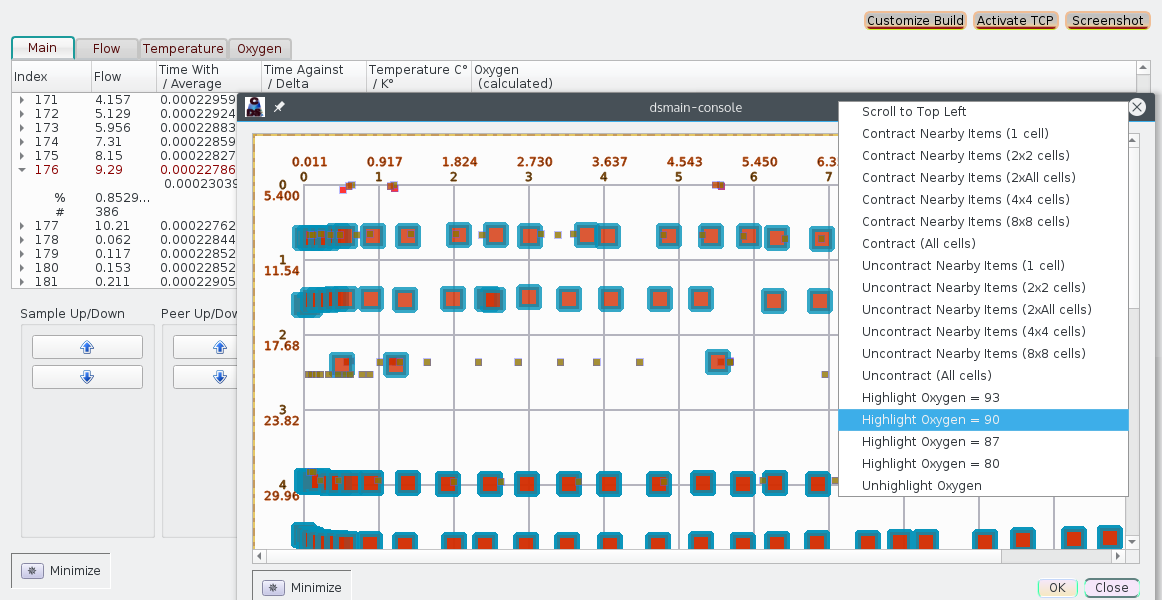
\includegraphics[width=180mm, 
    	trim={0mm 0mm 0mm 0mm},clip]
    	{pics/oxy.png}};
    
\end{tikzpicture}   
\end{figure}



\p{Diagram-based \MdsX{} notebooks can be implemented with 
different diagram-plotting engines; the default 
implementations support \Qt{} Charts (a built-in \Qt{} 
module) as well as the qtcustomplot and 
JKQCustomPlotter libaries.  In short, diagram-based 
notebooks need to implement subclasses of 
\MdsX{} frames for a navigation panel, graphics view, 
meta-procedure view, and data view, as well as a 
\q{\MdsX{} diagram} subclass occupying the diagram view.  
In this case, the primary responsibility of 
the meta-procedural layer is to interface with 
functionality provided by the diagram/plotting 
engine.  Since most coding details are derived from 
these engine's object models and classes, they lie 
mostly outside the scope of this paper.}

\p{Image-based notebooks, on the other hand, 
need to integrate several different 
areas of functionality.  As such, setting 
up the image view is only one step in 
constructing such a notebook; additional 
programming is needed to support image annotation, 
analysis, and feature extraction.  
In order to integrate these different layers 
of functionality, \MdsX{} provides a 
\q{Data Structure Protocol for Image-Analysis Networking} 
(\DSPIN{}) which defines communication rules 
between image-related software subsystems 
in Object-Oriented terms.  \DSPIN{} 
objects are comprised of four 
more specific objects or layers, describing 
different aspects of the shared image and 
how it should be processed.  These 
four layers are defined as follows:

\begin{description} 

\item[Metadata Layer]  This object presents 
metadata describing the image format and acquisition.  
If the surrounding \DSPIN{} object represents an 
image series (rather than a single image), the 
metadata object should also declare the 
size of the collection and how individual 
images should be referenced.  The metadata 
should include a file path or resource identifier 
asserting where the image can be acquired from 
(which in the case of a series can be a zipped 
folder or a list of resource paths).  More 
specific metadata depends on the image or images' 
graphical format; to properly load images in 
most formats (such as \PNG{}, \JPEG{}, \TIFF{}, 
and \DICOM{}) applications need to specify 
detail such as dimensions, resolution, and 
color depth.  Of course, some of this information 
is stored internally within the image file 
(depending on its format), but certain formats 
require some metadata to be shared along with 
the image itself (moreover, it is often convenient 
to have basic information available without needing 
to extract it from binary image data).  The details 
on which form of metadata are appropriate for 
which image format can be determined based 
on image-viewing code libraries, such as 
\textbf{libpng}, \textbf{libtiff}, or 
\DICOM{} clients.  If both end-points of a 
\DSPIN{} communication have the same 
libraries installed, the sending application 
will have a clear idea of how much supplemental 
data is needed over and above what will be 
read from image files directly.  If there 
are uncertainties in library alignment between 
the two end-points, the sending application should 
consider serializing a more detailed summary of 
the image providing any information that would 
ordinarily be read from the image file. 
  
\item[Annotation Layer]
Almost all image analysis --- whether done by 
humans or by softare --- results in either 
some form of statistical representation of 
an image's properties, or a complex of 
data which presents information about 
(and may visually overlay) the image, 
particularly in the form of annotations.  
Image annotations are arrows, line segments, 
or \TwoD{} closed shapes that call attention 
to some point or region inside the image, 
usually with some additional label or commentary.  
The basis of each annotation is therefore 
some zero-dimensional or two-dimensional 
region (or a set of zero-dimensional 
control points; or, occasionally, a one-dimensonsal  
line or curve), so annotations require a mechanism 
for designating regions.  The same 
issues apply to asserting feature-vectors 
with respect to an image region rather than 
the image as a whole; accordingly, 
both annotations and feature vectors 
can be seen as equivalent varieties of 
constructions which isolate and then 
define data structures on zero-, one-, 
and/or two-dimensional subimages 
(feature vectors on the entire image 
can accordingly be treated as a special 
case).    

\item[Contextual Layer]
Contextual information associated with an 
image can include metadata 
or supplemental details that are not 
directly relevant to the image, but 
convey facts about how the image connects 
to a broader context where it was obtained, 
and for what purpose.  An example of 
contextual data would be the part of 
\DICOM{} headers that include patient 
or clinical information, rather than 
metadata about image format or 
dimensions.  


\item[Procedural Layer]

\end{description}
}


\p{In \MdsX{}, \DSPIN{} objects are 
associated with image-based notebooks in 
that the notebook components 
(the navigation panel and graphics, data, 
and meta-procedural controllers) jointly refer 
to a common \DSPIN{} object for all 
image-related data.  Image-analysis routines 
conducted within the notebook then may yield 
additional data structures bundled into the 
overarching \DSPIN{} object.  This 
overarching object can then be exported or 
saved, alongside (and as an extension of) 
notebook state.}

\p{Analytic operations available through an 
image-based notebook may be provided by 
the notebook itself, or by a host application 
where \MdsX{} is embedded.  In the latter 
case, the notebook needs to construct the 
proper calls to the host application, using 
the meta-procedural controller as a bridge 
to ambient capabilities.  For instance, if 
an \MdsX{} notebook is developed as a plugin 
to \CaPTk{}, the notebook would interface 
with the host \CaPTk{} application via the 
formats and programming constructs which 
\CaPTk{} recognizes (specifically, 
the Common Workflow Language and the 
\Qt{} signal/slot mechanism).  
This specific scenario --- embedding \MdsX{} 
in \CaPTk{} --- is employed as a demonstration 
and case-study for embedding notebooks 
in host application in general.  
The \CaPTk{} workflow protocol also forms a 
basis for the meta-procedural view and 
controllers, discussed next.}

\section[MdsX Meta-Procedure Controllers]{\protect\lsMdsX{} Meta-Procedure Controllers}

\p{The meta-procedural layer of an \MdsX{} notebook 
is responsible for handling events generated 
by a corresponding navigational panel, or at 
least those events which have a 
non-trivial impact on notebook/session 
state and data.  The visual representation of 
meta-procedural commands and history is 
provided by a meta-procedural \q{view,} which 
is normally invisible, but notebooks may 
choose to allow users to \q{unhide} this view.  
The meta-procedural controller is responsible 
for generating the meta-procedural view (if 
applicable) and responding to user events 
within this view; it is also responsible for 
maintaining an inventory of objects summarizing 
available metaprocedures, \GUI{} elements, 
and the mappings between them.}

\p{In general, the \GUI{} elements in these 
meta-procedural mappings are referred to as 
\q{visual objects,} and are represented 
in the meta-procedural controller context via 
application-unique identifiers (not raw pointers).  
Similarly, \q{meta-procedural objects} encapsulate 
information about meta-procedures themselves.  
This controller does not directly connect 
\GUI{} events to event handlers; instead, it 
receives information about these connections when 
the notebook is loaded.  The controller is however 
responsible for implementing \textit{incremental 
execution} wrapping event callbacks (or any other 
relevant procedure).  Incremental execution 
means that the controller may create 
temporary \q{execution contexts} and incrementally 
build up the data which, given a sufficiently 
complete \q{marking,} can lead to the 
meta-procedure being \q{fired.}  Each 
preliminary stage --- that is, each pre-firing 
addition to the execution context --- may in 
turn be generated by events originating elsewhere 
in the application (canonically, the 
navigation panel), and the meta-procedural controller 
should model both the history of these pre-firing stages 
and the origin and nature of the events which 
triggered them.  An execution context 
may then be \textit{reified}, representing the 
cumulative pre-firing stages as a data structure 
that can be matched to a meta-procedure's 
outcomes: for example, noting the 
inputs or steps producing the specific appearance 
of a diagram or image in the graphics view, 
or the parameters configured to instantiate 
a workflow model.  Reified meta-procedural 
execution contexts can then be shared as 
objects with components responsible for 
sharing or preserving information about the 
notebook.  For instance, a notebook graphic may be 
included in a publication; the reified context 
could then be associated with that image as an 
annotation, and used to reconstruct notebook 
state if the notebook is launched from a 
document viewer in the context of the 
published graphic.}

\p{In general, the information represented 
by the meta-procedural controller is not only 
relevant for the reactive operations of the 
notebook, responding to user actions; 
it also serves to document the notebook's 
properties, and potentially to connect 
the notebook with data sets and/or 
publications.  Many operations which can be 
performed within a notebook are associated 
with a given scientific or theoretical 
concept, or a statistical parameter modeled 
within a data set.  As such, it is possible 
for the notebook to maintain a list of these 
concepts, so as to create an interactive 
glossary or to interoperate with a document 
viewer.  For instance, Figure~\ref{fig:oxy} shows a 
context-menu action based on the concept 
of \q{oxygenated air flow,} which is also 
discussed in the scientific article 
on which the depicted data set is based.  
This concept also has a visual expression in 
one table column shown (in the background) on 
Figure~\ref{fig:oxy}.  As demonstrated 
in Figure~\ref{fig:about}, the data-set application includes 
code to explain technical concepts in pop-up 
dialog boxes, and also to link to the 
page/paragraph in the article where that correspinding 
concept is first (or most thoroughly) defined/mentioned.  
Establishing these conceptual connections 
between an \MdsX{} notebook, data set, and 
technical publication is facilitated by 
annotating both meta-procedural capabilities 
and \GUI{} elements with references to 
relevant technical/scientific concepts; these 
annotations, when defined, are represented through the 
meta-procedural controller.}

\begin{figure}

\caption{Linking Dataset Applications to Publications}
\label{fig:about}

\begin{tikzpicture}

\node[inner sep=0pt] (x1) at (0,0)
    {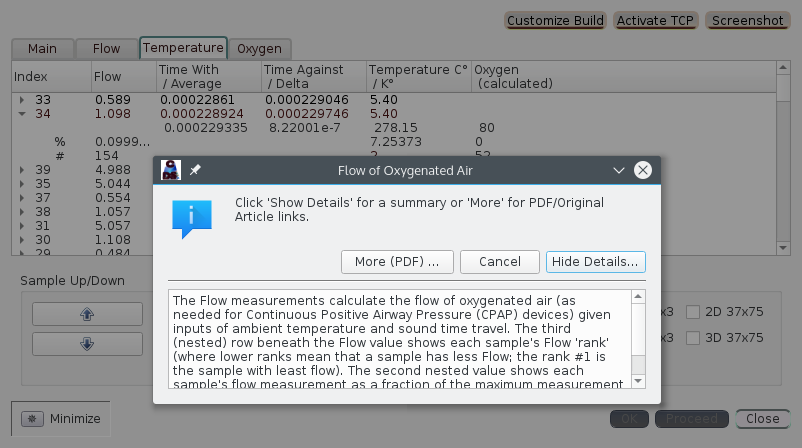
\includegraphics[width=180mm, 
    	trim={0mm 0mm 0mm 0mm},clip]
    	{pics/about.png}};

\end{tikzpicture}    
\end{figure}



\p{}


\end{document}
